\MainChapter{Pruebas}{\topBanner}\label{cap:pruebas}
\vspace*{0.7cm}

En esta sección se describe el proceso de verificación de la solución de servicio de directorio implementada, con el propósito de determinar el grado de cumplimiento de los requisitos establecidos. Primero se presenta la metodología de pruebas, incluyendo los tipos de pruebas, las condiciones de ejecución y el diseño de los casos de prueba. Luego se detallan los resultados de la ejecución de nueve pruebas que abordan la integración y autenticación centralizada, la autorización diferenciada, la gestión del ciclo de vida de cuentas, las políticas de seguridad, la trazabilidad, el control de acceso, la replicación, la continuidad ante fallas y la recuperación del servicio. Finalmente, se presenta la evaluación consolidada del cumplimiento de requisitos.

\section{Metodología}
La fase de pruebas tuvo como propósito verificar el funcionamiento de la solución de servicio de directorio implementada y determinar el grado de cumplimiento de los requisitos establecidos.
La evaluación abarcó la solución como un conjunto, considerando a FreeIPA como componente central para la gestión de identidades y su integración con OpenVPN, OpenProject y Xen Orchestra, así como la configuración de réplica implementada para proporcionar continuidad del servicio.

Las pruebas se diseñaron a partir de los comportamientos que debían ser demostrados por la solución, en lugar de establecer una correspondencia individual entre cada requisito y un caso de prueba. De esta manera, una misma prueba proporciona evidencia para uno o varios requisitos cuando estos involucran comportamientos relacionados. Este enfoque permite evitar la repetición de procedimientos y evidencias, manteniendo una relación directa entre los resultados obtenidos y los requisitos evaluados.

La ejecución tuvo lugar en escenarios controlados, en los cuales quedaron definidas previamente las condiciones del entorno, los datos de prueba y el comportamiento esperado. Posteriormente se ejecutó un conjunto de acciones reproducibles y se registró el comportamiento observado. Los resultados obtenidos fueron comparados con los resultados esperados para determinar el estado de cada prueba.

La evaluación utilizó tres estados:
\begin{itemize}
	\item \textbf{Cumple:} el comportamiento observado coincide con el resultado esperado y proporciona evidencia suficiente del cumplimiento del requisito asociado.
	\item \textbf{Cumple parcialmente:} la solución proporciona parte de la funcionalidad requerida, pero presenta limitaciones respecto al alcance establecido para el requisito.
	\item \textbf{No cumple:} la funcionalidad requerida no se encuentra disponible o no fue posible demostrar su funcionamiento durante las pruebas.
\end{itemize}

Las evidencias obtenidas durante la ejecución permitieron relacionar los resultados de las pruebas con los requisitos R-01 a R-08 y establecer el nivel de cumplimiento de la solución.

\subsection{Tipos de pruebas}
Las pruebas se organizaron de acuerdo con el comportamiento que se pretendía verificar. Se contemplaron los siguientes tipos:
\begin{itemize}
	\item \textbf{Pruebas funcionales:} permiten verificar las operaciones relacionadas con la gestión de identidades y credenciales, incluyendo la creación, actualización, habilitación, deshabilitación, revocación y expiración de cuentas, así como la aplicación de las políticas configuradas.
	\item \textbf{Pruebas de integración:} permiten comprobar que OpenVPN, OpenProject y Xen Orchestra utilizan el servicio de directorio para realizar la gestión y autenticación de las identidades, verificando que las credenciales centralizadas pueden ser utilizadas de acuerdo con los permisos definidos para cada sistema.
	\item \textbf{Pruebas de seguridad y control de acceso:} permiten comprobar la aplicación de las políticas de credenciales y la autorización diferenciada mediante grupos y permisos, incluyendo escenarios de acceso permitido y rechazado.
	\item \textbf{Pruebas de auditoría:} permiten verificar la generación y consulta de registros asociados a actividades relevantes de gestión de identidades, autenticación y acceso.
	\item \textbf{Pruebas de disponibilidad y continuidad:} permiten verificar la sincronización entre el servidor principal y la réplica, el comportamiento de la solución ante la indisponibilidad del servidor principal y la recuperación posterior de la infraestructura.
\end{itemize}

\subsection{Condición de ejecución}
Las pruebas se ejecutaron sobre el entorno construido durante la fase de implementación. Se conservaron las configuraciones necesarias para reproducir el funcionamiento habitual de la solución, evitando realizar modificaciones adicionales que pudieran alterar el comportamiento que se pretendía evaluar.

\subsection{Diseño de los casos de prueba}
Los casos de prueba son diseñados a partir de los comportamientos que deben ser demostrados por la solución. Los casos son asociados a uno o varios requisitos cuando el mismo escenario permite obtener evidencia suficiente para su evaluación.

Para mantener una ejecución uniforme, cada caso de prueba utiliza la siguiente estructura, definida en la \autoref{tab:estructura-casos-prueba}:

\begingroup
\fontsize{8.5pt}{9.5pt}\selectfont
\renewcommand{\arraystretch}{1.3}
\setlength{\tabcolsep}{4pt}

\begin{longtable}{|
	>{\raggedright\arraybackslash}p{4.0cm}|
	>{\raggedright\arraybackslash}p{9.5cm}|}

	\caption{Estructura de los casos de prueba}
	\label{tab:estructura-casos-prueba}
	\\
	\hline
	\rowcolor[gray]{0.85}
	\textbf{Campo}             &
	\textbf{Descripción}
	\\
	\hline
	\endfirsthead

	\hline
	\rowcolor[gray]{0.85}
	\textbf{Campo}             &
	\textbf{Descripción}
	\\
	\hline
	\endhead

	ID                         & Identificador único asignado al caso de prueba.                                                                \\ \hline
	Nombre                     & Denominación que describe de forma breve el comportamiento evaluado.                                           \\ \hline
	Requisitos asociados       & Requisitos que pueden ser evaluados mediante la prueba.                                                        \\ \hline
	Objetivo                   & Comportamiento específico que se pretende verificar.                                                           \\ \hline
	Resultado esperado         & Comportamiento que debería producirse si la solución funciona de acuerdo con lo establecido.                   \\ \hline
	Precondiciones             & Condiciones que deben cumplirse antes de iniciar la prueba.                                                    \\ \hline
	Datos de prueba            & Usuarios, grupos, credenciales u otros elementos utilizados durante la ejecución.                              \\ \hline
	Procedimiento y evidencias & Secuencia de los procedimientos realizados, indicando cada literal y acompañándolo de su respectiva evidencia. \\ \hline
	Estado                     & Clasificación final de la prueba como cumple, cumple parcialmente o no cumple.                                 \\ \hline
	Observaciones              & Información adicional relevante sobre la ejecución, incidencias o limitaciones identificadas.                  \\ \hline
\end{longtable}
\endgroup
\normalsize

El resultado esperado quedó definido antes de ejecutar cada prueba, con el propósito de disponer de un criterio objetivo de comparación. Una vez finalizada la ejecución, se documentó el resultado obtenido y se incorporaron las evidencias correspondientes.

La asignación de requisitos no implica que cada requisito tenga un caso de prueba independiente. Por ejemplo, una prueba de autorización diferenciada permite demostrar simultáneamente que las identidades son gestionadas de forma centralizada y que los permisos se mantienen diferenciados entre OpenVPN, OpenProject y Xen Orchestra. De esta forma, se evita repetir la creación de usuarios, configuraciones y procedimientos cuando estos ya han sido comprobados mediante otra prueba.

La batería de pruebas se organizó en torno a los siguientes escenarios principales, presentados en la \autoref{tab:bateria-pruebas}:

\begingroup
\fontsize{8.5pt}{9.5pt}\selectfont
\renewcommand{\arraystretch}{1.3}
\setlength{\tabcolsep}{4pt}

\begin{longtable}{|
	>{\raggedright\arraybackslash}p{1.5cm}|
	>{\raggedright\arraybackslash}p{4.0cm}|
	>{\raggedright\arraybackslash}p{2.5cm}|
	>{\raggedright\arraybackslash}p{5.5cm}|}

	\caption{Escenarios principales de la batería de pruebas}
	\label{tab:bateria-pruebas}
	\\
	\hline
	\rowcolor[gray]{0.85}
	\textbf{ID}                   &
	\textbf{Caso de prueba}       &
	\textbf{Requisitos asociados} &
	\textbf{Propósito principal}
	\\
	\hline
	\endfirsthead

	\hline
	\rowcolor[gray]{0.85}
	\textbf{ID}                   &
	\textbf{Caso de prueba}       &
	\textbf{Requisitos asociados} &
	\textbf{Propósito principal}
	\\
	\hline
	\endhead

	PT-01                         & Integración y autenticación centralizada            & R-01, R-08 & Verificar el uso de las identidades de FreeIPA en los tres servicios.                        \\ \hline
	PT-02                         & Autorización diferenciada mediante grupos           & R-01, R-04 & Comprobar que los permisos se mantienen diferenciados por sistema.                           \\ \hline
	PT-03                         & Gestión del ciclo de vida de las cuentas            & R-02       & Verificar las operaciones principales sobre las identidades y su efecto sobre el acceso.     \\ \hline
	PT-04                         & Aplicación de políticas de seguridad y credenciales & R-03, R-06 & Comprobar las restricciones configuradas sobre las credenciales y su aplicación.             \\ \hline
	PT-05                         & Registro y trazabilidad de actividades              & R-05       & Verificar la generación y consulta de registros relacionados con identidades y accesos.      \\ \hline
	PT-06                         & Revisión de permisos y control de acceso            & R-04       & Verificar la capacidad de consultar y revisar las autorizaciones configuradas.               \\ \hline
	PT-07                         & Replicación y sincronización                        &            & Comprobar la sincronización de identidades entre el servidor principal y la réplica.         \\ \hline
	PT-08                         & Continuidad ante falla del servidor principal       &            & Verificar que los servicios integrados pueden continuar operando mediante la réplica.        \\ \hline
	PT-09                         & Recuperación y resincronización                     &            & Comprobar la recuperación del servidor principal y el restablecimiento de la sincronización. \\ \hline
\end{longtable}
\endgroup
\normalsize

Las pruebas PT-07, PT-08 y PT-09 no se asociaron directamente con un requisito R-01--R-08, debido a que evalúan características de la arquitectura implementada relacionadas con la replicación, disponibilidad y recuperación. No obstante, sus resultados se consideran en la evaluación general de la solución, debido a que permiten verificar la continuidad del servicio de directorio sobre el cual dependen los sistemas integrados.

La ejecución detallada de cada caso se presenta en la siguiente sección, incorporando el procedimiento realizado, los resultados obtenidos y las evidencias que permiten sustentar posteriormente la evaluación de los requisitos.

\section{Ejecución de las pruebas}

\subsection{PT-01 - Integración y autenticación centralizada}
\textbf{Requisitos asociados:} R-01, R-08.\\
\textbf{Objetivo:} Verificar la integración del servicio de directorio con OpenVPN, OpenProject y Xen Orchestra, comprobando que las identidades gestionadas en FreeIPA pueden utilizarse para la autenticación en los tres servicios. Asimismo, se busca evidenciar que el directorio constituye un punto central para la gestión de las identidades utilizadas por los sistemas integrados.\\
\textbf{Resultado esperado:} La cuenta gestionada en FreeIPA debe permitir la autenticación en los tres servicios integrados, siempre que cumpla las condiciones de acceso establecidas para cada uno. El uso de una misma identidad en los diferentes sistemas debe evidenciar que FreeIPA funciona como servicio central de gestión de identidades, sin requerir la creación de una identidad independiente para cada servicio.\\
\textbf{Precondiciones:}
\begin{itemize}
	\item El servidor principal de FreeIPA se encuentra operativo.
	\item La cuenta de prueba se encuentra registrada en FreeIPA.
	\item Las integraciones de OpenVPN, OpenProject y Xen Orchestra con FreeIPA se encuentran configuradas.
	\item Los tres servicios se encuentran disponibles.
	\item La cuenta de prueba dispone de los permisos necesarios para realizar el acceso a cada servicio.
\end{itemize}
\textbf{Datos de prueba:} Se utilizó una cuenta de usuario previamente creada en FreeIPA. La misma identidad fue empleada para realizar los intentos de autenticación en los tres servicios integrados, con el propósito de comprobar el uso de las credenciales centralizadas.\\
\textbf{Procedimiento y evidencias:}
\begin{enumerate}
	\item \textbf{Verificación de la identidad en FreeIPA:} Se verificó en FreeIPA la existencia de la cuenta de prueba y su estado, comprobando que la identidad se encontrara registrada y habilitada para su utilización en los servicios integrados, como se observa en la \autoref{fig:figura-1}.
	      \begin{figure}[H]
		      \centering
		      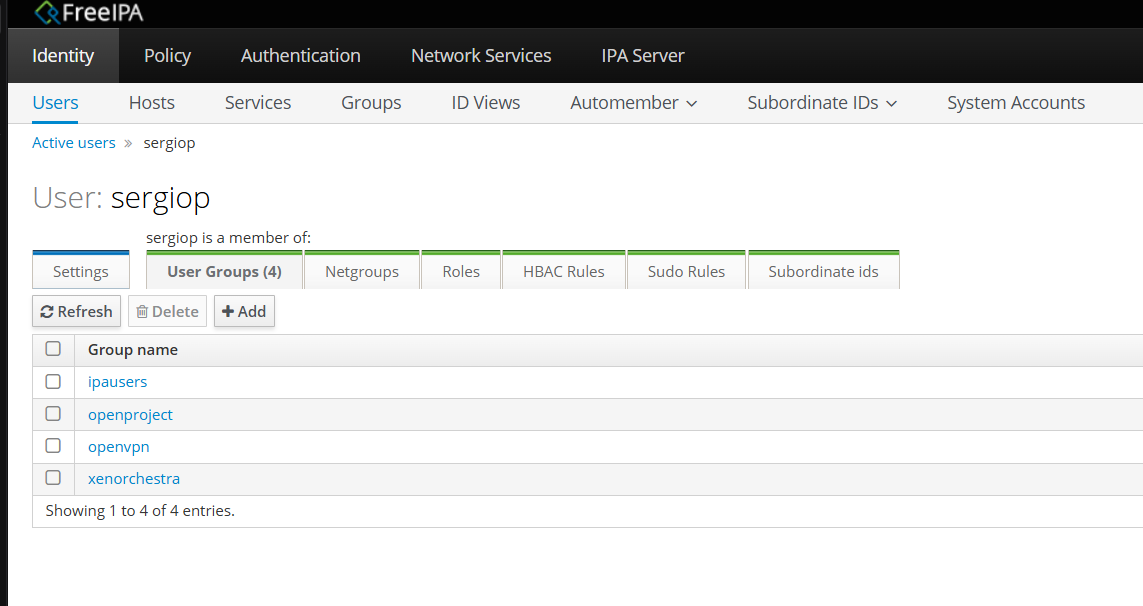
\includegraphics[width=0.85\textwidth]{imagenes/figuras/II-desarrollo-metodologico/pruebas/figura-1.png}
		      \caption{Cuenta de prueba registrada y habilitada en FreeIPA.}
		      \label{fig:figura-1}
	      \end{figure}

	\item \textbf{Validación de la autenticación en OpenVPN:} Se utilizaron las credenciales de la cuenta de prueba para realizar la autenticación mediante OpenVPN. Una vez realizado el proceso, se verificó el resultado de la conexión para comprobar que las credenciales gestionadas por FreeIPA fueran aceptadas por el servicio, tal como se muestra en la \autoref{fig:figura-2}.
	      \begin{figure}[H]
		      \centering
		      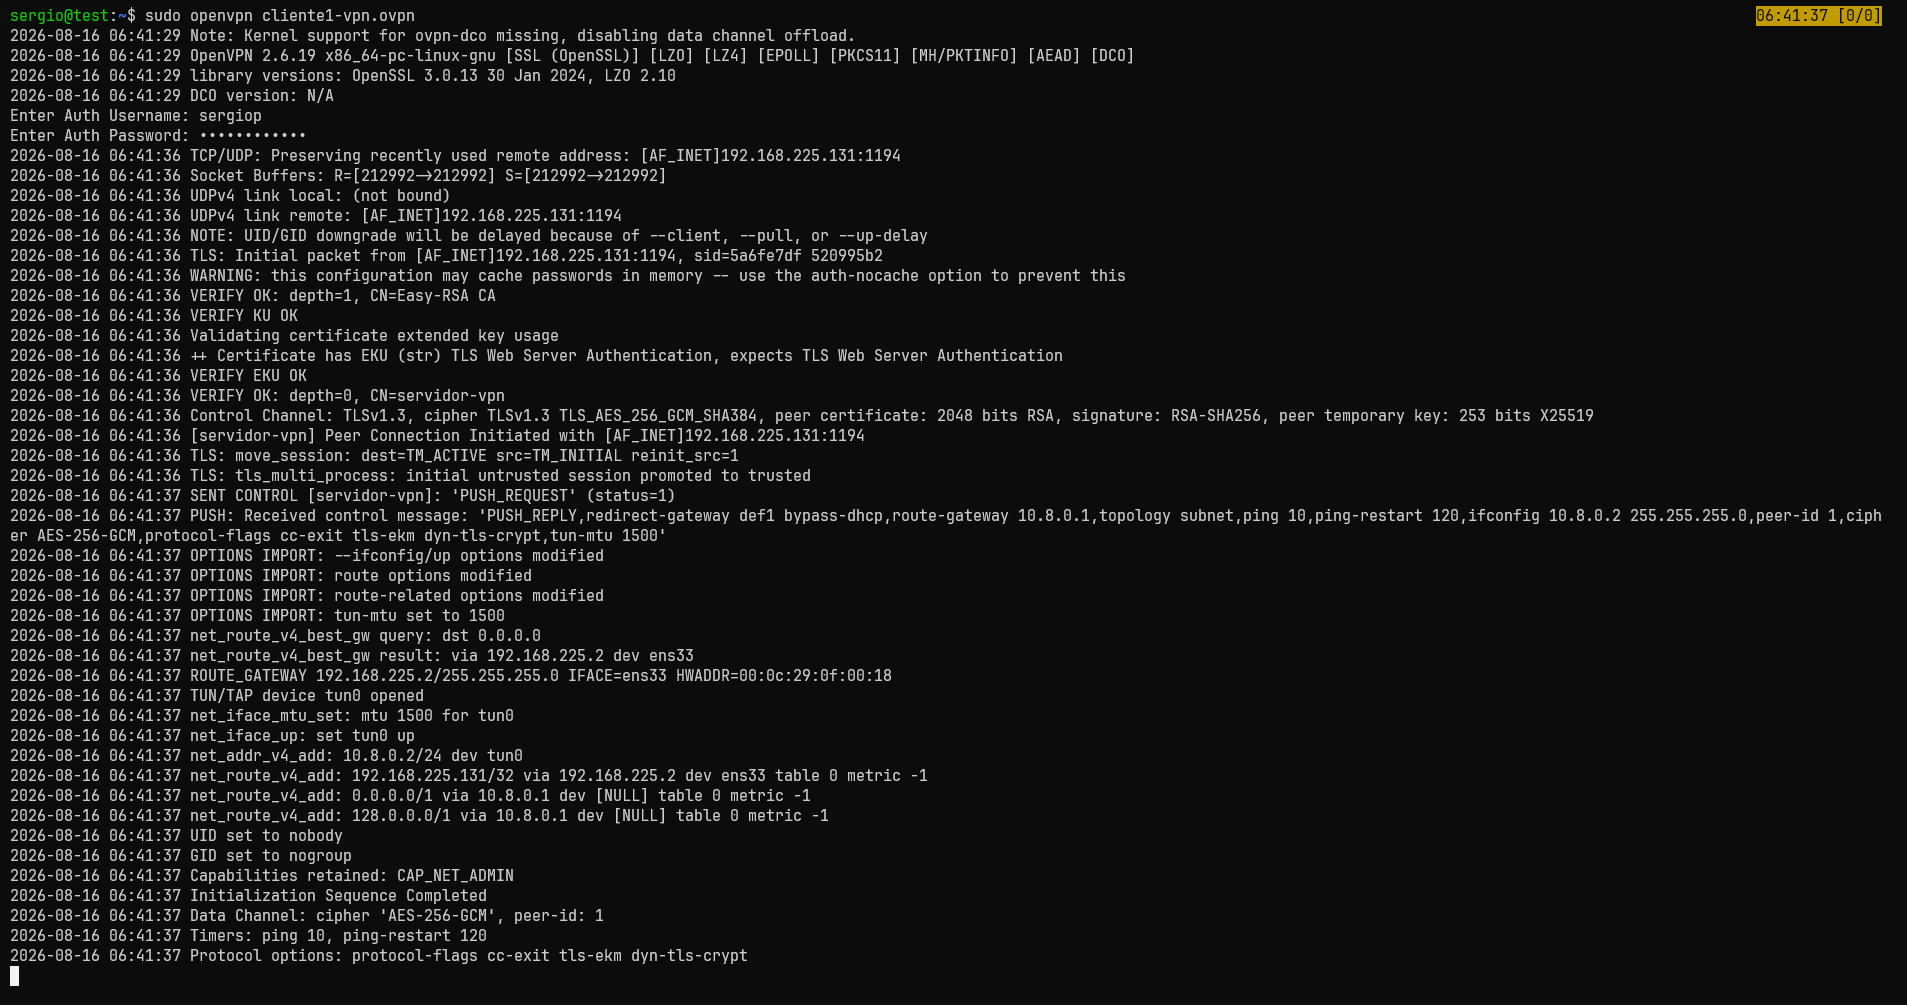
\includegraphics[width=0.85\textwidth]{imagenes/figuras/II-desarrollo-metodologico/pruebas/figura-2.png}
		      \caption{Autenticación de la cuenta de prueba mediante OpenVPN.}
		      \label{fig:figura-2}
	      \end{figure}

	\item \textbf{Validación de la autenticación en OpenProject:} Se utilizaron las mismas credenciales de la cuenta de prueba para realizar la autenticación en OpenProject. Posteriormente, se verificó el acceso obtenido en el sistema, como se observa en la \autoref{fig:figura-3}.
	      \begin{figure}[H]
		      \centering
		      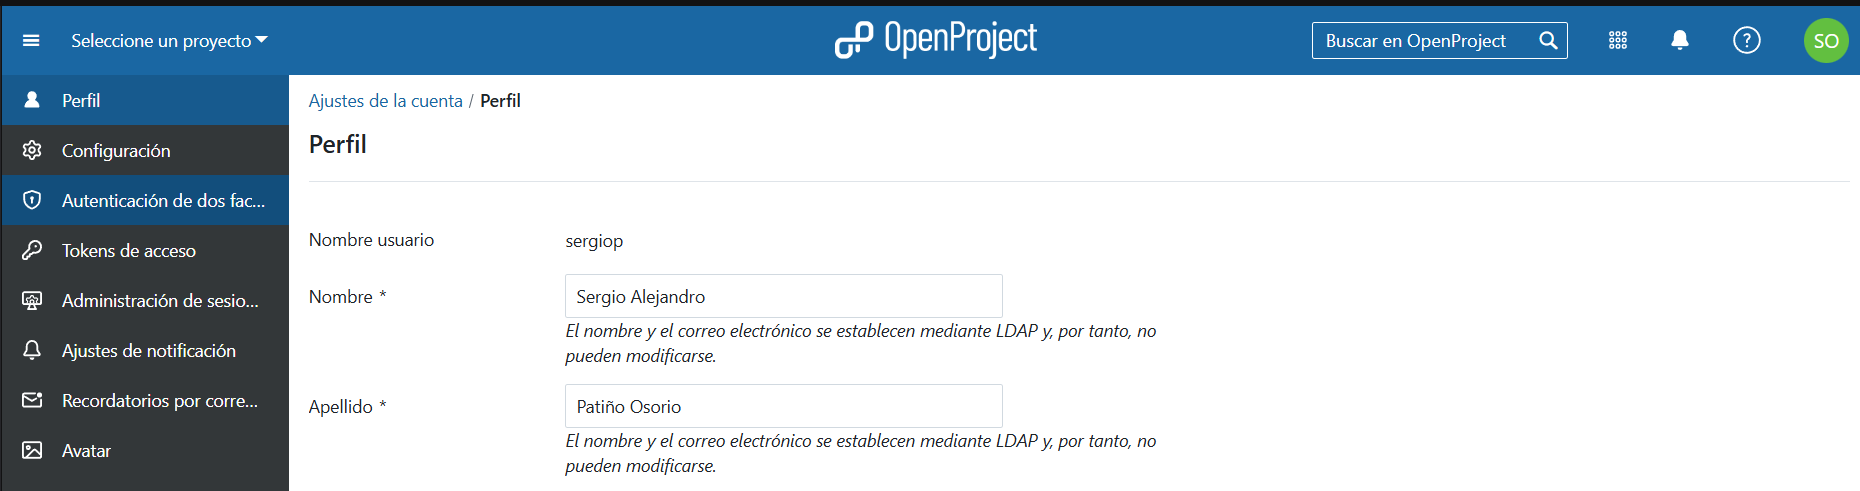
\includegraphics[width=0.85\textwidth]{imagenes/figuras/II-desarrollo-metodologico/pruebas/figura-3.png}
		      \caption{Autenticación de la cuenta de prueba en OpenProject.}
		      \label{fig:figura-3}
	      \end{figure}

	\item \textbf{Validación de la autenticación en Xen Orchestra:} Finalmente, se utilizaron las mismas credenciales de la cuenta de prueba para realizar la autenticación en Xen Orchestra. Se verificó el resultado del proceso y el acceso al sistema, tal como se presenta en la \autoref{fig:figura-4}.
	      \begin{figure}[H]
		      \centering
		      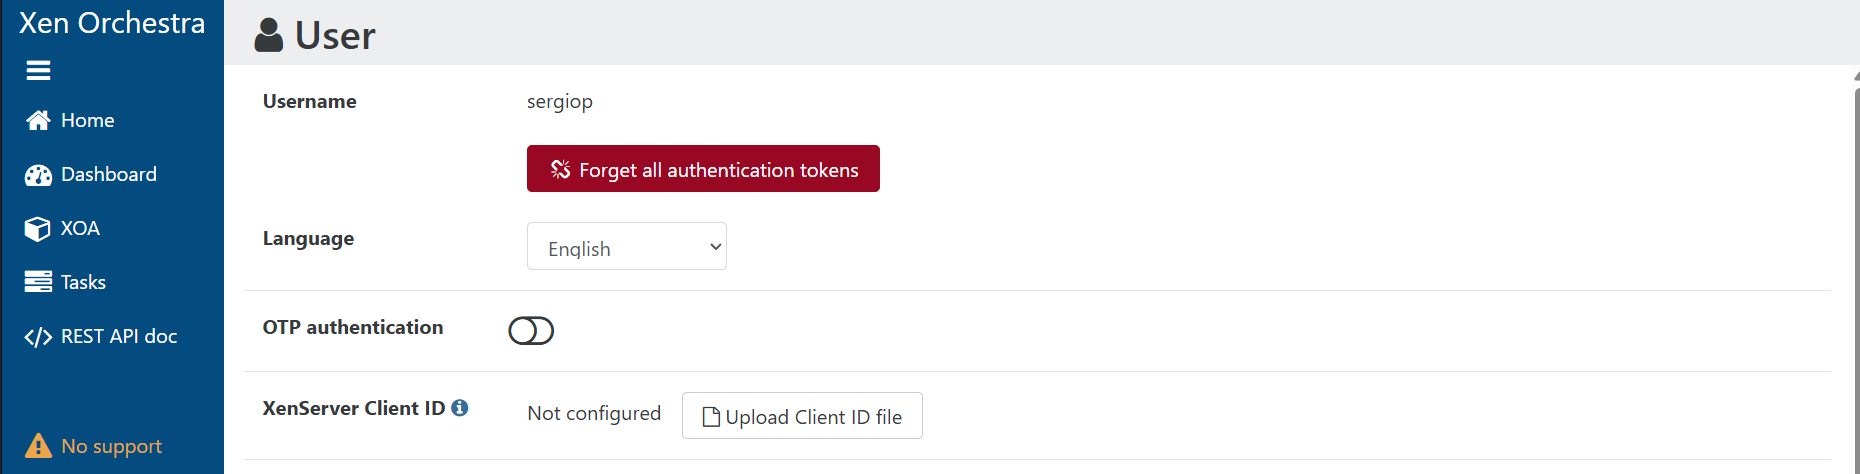
\includegraphics[width=0.85\textwidth]{imagenes/figuras/II-desarrollo-metodologico/pruebas/figura-4.png}
		      \caption{Autenticación de la cuenta de prueba en Xen Orchestra.}
		      \label{fig:figura-4}
	      \end{figure}
\end{enumerate}
\textbf{Estado:} Cumple.\\
\textbf{Observaciones:} La prueba permitió comprobar el uso de FreeIPA como punto central para la gestión de las identidades utilizadas por los tres servicios integrados. La utilización de una misma cuenta en OpenVPN, OpenProject y Xen Orchestra permitió demostrar la centralización de las identidades contemplada en R-01.
Asimismo, la integración de FreeIPA con los tres sistemas permitió evidenciar su utilización como servicio común ante diferentes sistemas, aportando evidencia al cumplimiento de R-08.

\subsection{PT-02 - Autorización diferenciada mediante grupos}
\textbf{Requisitos asociados:} R-01, R-04.\\
\textbf{Objetivo:} Verificar que la pertenencia de los usuarios a grupos de autorización definidos en FreeIPA permite establecer permisos diferenciados entre OpenVPN, OpenProject y Xen Orchestra, comprobando que cada cuenta puede acceder al servicio para el cual se encuentra autorizada y que el acceso a los demás servicios es rechazado.\\
\textbf{Resultado esperado:} Cada cuenta debe poder acceder únicamente al servicio asociado al grupo al que pertenece. Los intentos de acceso a los demás servicios deben ser rechazados.

Por tanto, el comportamiento esperado se resume en la \autoref{tab:pt02-comportamiento-esperado}:

\begingroup
\fontsize{8.5pt}{9.5pt}\selectfont
\renewcommand{\arraystretch}{1.3}
\setlength{\tabcolsep}{4pt}

\begin{longtable}{|
	>{\raggedright\arraybackslash}p{4.5cm}|
	>{\raggedright\arraybackslash}p{3.0cm}|
	>{\raggedright\arraybackslash}p{3.0cm}|
	>{\raggedright\arraybackslash}p{3.0cm}|}

	\caption{Comportamiento esperado por servicio según el grupo de autorización}
	\label{tab:pt02-comportamiento-esperado}
	\\
	\hline
	\rowcolor[gray]{0.85}
	\textbf{Cuenta}                &
	\textbf{OpenVPN}               &
	\textbf{OpenProject}           &
	\textbf{Xen Orchestra}
	\\
	\hline
	\endfirsthead

	\hline
	\rowcolor[gray]{0.85}
	\textbf{Cuenta}                &
	\textbf{OpenVPN}               &
	\textbf{OpenProject}           &
	\textbf{Xen Orchestra}
	\\
	\hline
	\endhead

	Cuenta 1 - Grupo OpenVPN       & Permitido & Rechazado & Rechazado \\ \hline
	Cuenta 2 - Grupo OpenProject   & Rechazado & Permitido & Rechazado \\ \hline
	Cuenta 3 - Grupo Xen Orchestra & Rechazado & Rechazado & Permitido \\ \hline
\end{longtable}
\endgroup
\normalsize

Este comportamiento permite comprobar que las identidades se gestionan de manera centralizada, mientras que la autorización se mantiene diferenciada según el sistema.\\
\textbf{Precondiciones:}
\begin{itemize}
	\item El servidor de FreeIPA se encuentra operativo.
	\item Las cuentas de prueba se encuentran creadas y habilitadas en FreeIPA.
	\item Los grupos de autorización para OpenVPN, OpenProject y Xen Orchestra se encuentran configurados.
	\item Las integraciones de los tres servicios con FreeIPA se encuentran operativas.
	\item Cada cuenta de prueba pertenece únicamente al grupo correspondiente al servicio para el cual se encuentra autorizada.
\end{itemize}
\textbf{Datos de prueba:} Se utilizaron tres cuentas gestionadas centralmente en FreeIPA. Cada una fue asociada a un grupo de autorización diferente, según se presenta en la \autoref{tab:pt02-datos-prueba}:

\begingroup
\fontsize{8.5pt}{9.5pt}\selectfont
\renewcommand{\arraystretch}{1.3}
\setlength{\tabcolsep}{4pt}

\begin{longtable}{|
	>{\raggedright\arraybackslash}p{2.5cm}|
	>{\raggedright\arraybackslash}p{2.5cm}|
	>{\raggedright\arraybackslash}p{4.0cm}|
	>{\raggedright\arraybackslash}p{4.5cm}|}

	\caption{Cuentas y grupos de autorización asignados para PT-02}
	\label{tab:pt02-datos-prueba}
	\\
	\hline
	\rowcolor[gray]{0.85}
	\textbf{Cuenta}                &
	\textbf{Usuario}               &
	\textbf{Grupo de autorización} &
	\textbf{Servicio autorizado}
	\\
	\hline
	\endfirsthead

	\hline
	\rowcolor[gray]{0.85}
	\textbf{Cuenta}                &
	\textbf{Usuario}               &
	\textbf{Grupo de autorización} &
	\textbf{Servicio autorizado}
	\\
	\hline
	\endhead

	Cuenta 1                       & pedrom  & Grupo openvpn      & OpenVPN       \\ \hline
	Cuenta 2                       & juang   & Grupo openproject  & OpenProject   \\ \hline
	Cuenta 3                       & sergiop & Grupo xenorchestra & Xen Orchestra \\ \hline
\end{longtable}
\endgroup
\normalsize

La tercera cuenta correspondió al usuario utilizado en PT-01, cuya pertenencia a grupos fue modificada previamente para que únicamente permaneciera asociada al grupo de Xen Orchestra.\\
\textbf{Procedimiento:}
\begin{enumerate}
	\item \textbf{Verificación de la pertenencia a los grupos:} Se consultó en FreeIPA la configuración de las tres cuentas de prueba, verificando que cada una perteneciera únicamente al grupo de autorización correspondiente al servicio para el cual se encontraba habilitada, como se muestra en la \autoref{fig:figura-5}.
	      \begin{figure}[H]
		      \centering
		      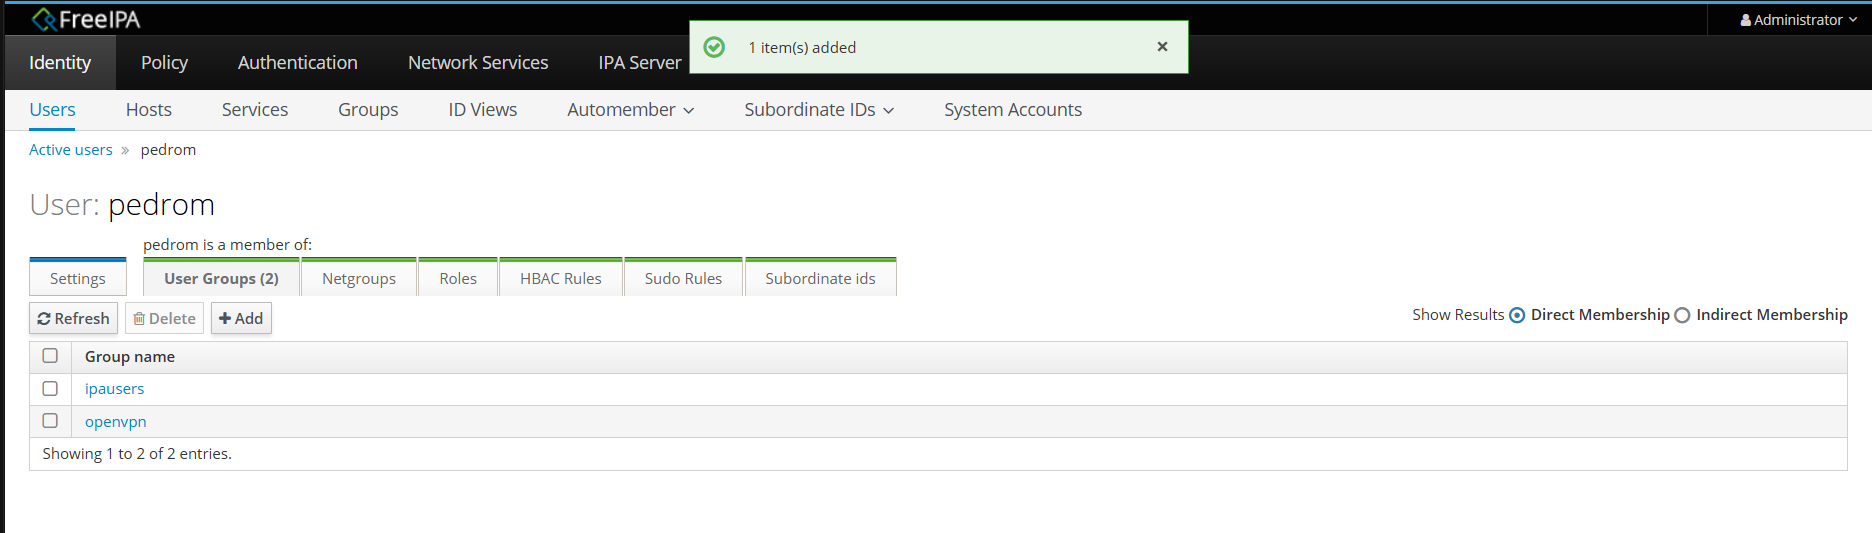
\includegraphics[width=0.85\textwidth]{imagenes/figuras/II-desarrollo-metodologico/pruebas/figura-5.png}
		      \caption{Pertenencia de las cuentas de prueba a los grupos de autorización en FreeIPA.}
		      \label{fig:figura-5}
	      \end{figure}

	\item \textbf{Validación del usuario autorizado para OpenVPN:} Se utilizaron las credenciales de la cuenta 1 para realizar intentos de autenticación en los tres servicios. El acceso a OpenVPN fue utilizado para comprobar el permiso correspondiente al grupo al que pertenecía la cuenta, mientras que los intentos realizados en OpenProject y Xen Orchestra permitieron comprobar el comportamiento ante servicios para los cuales no contaba con autorización. Los resultados se ilustran en la \autoref{fig:figura-6}.
	      \begin{figure}[H]
		      \centering
		      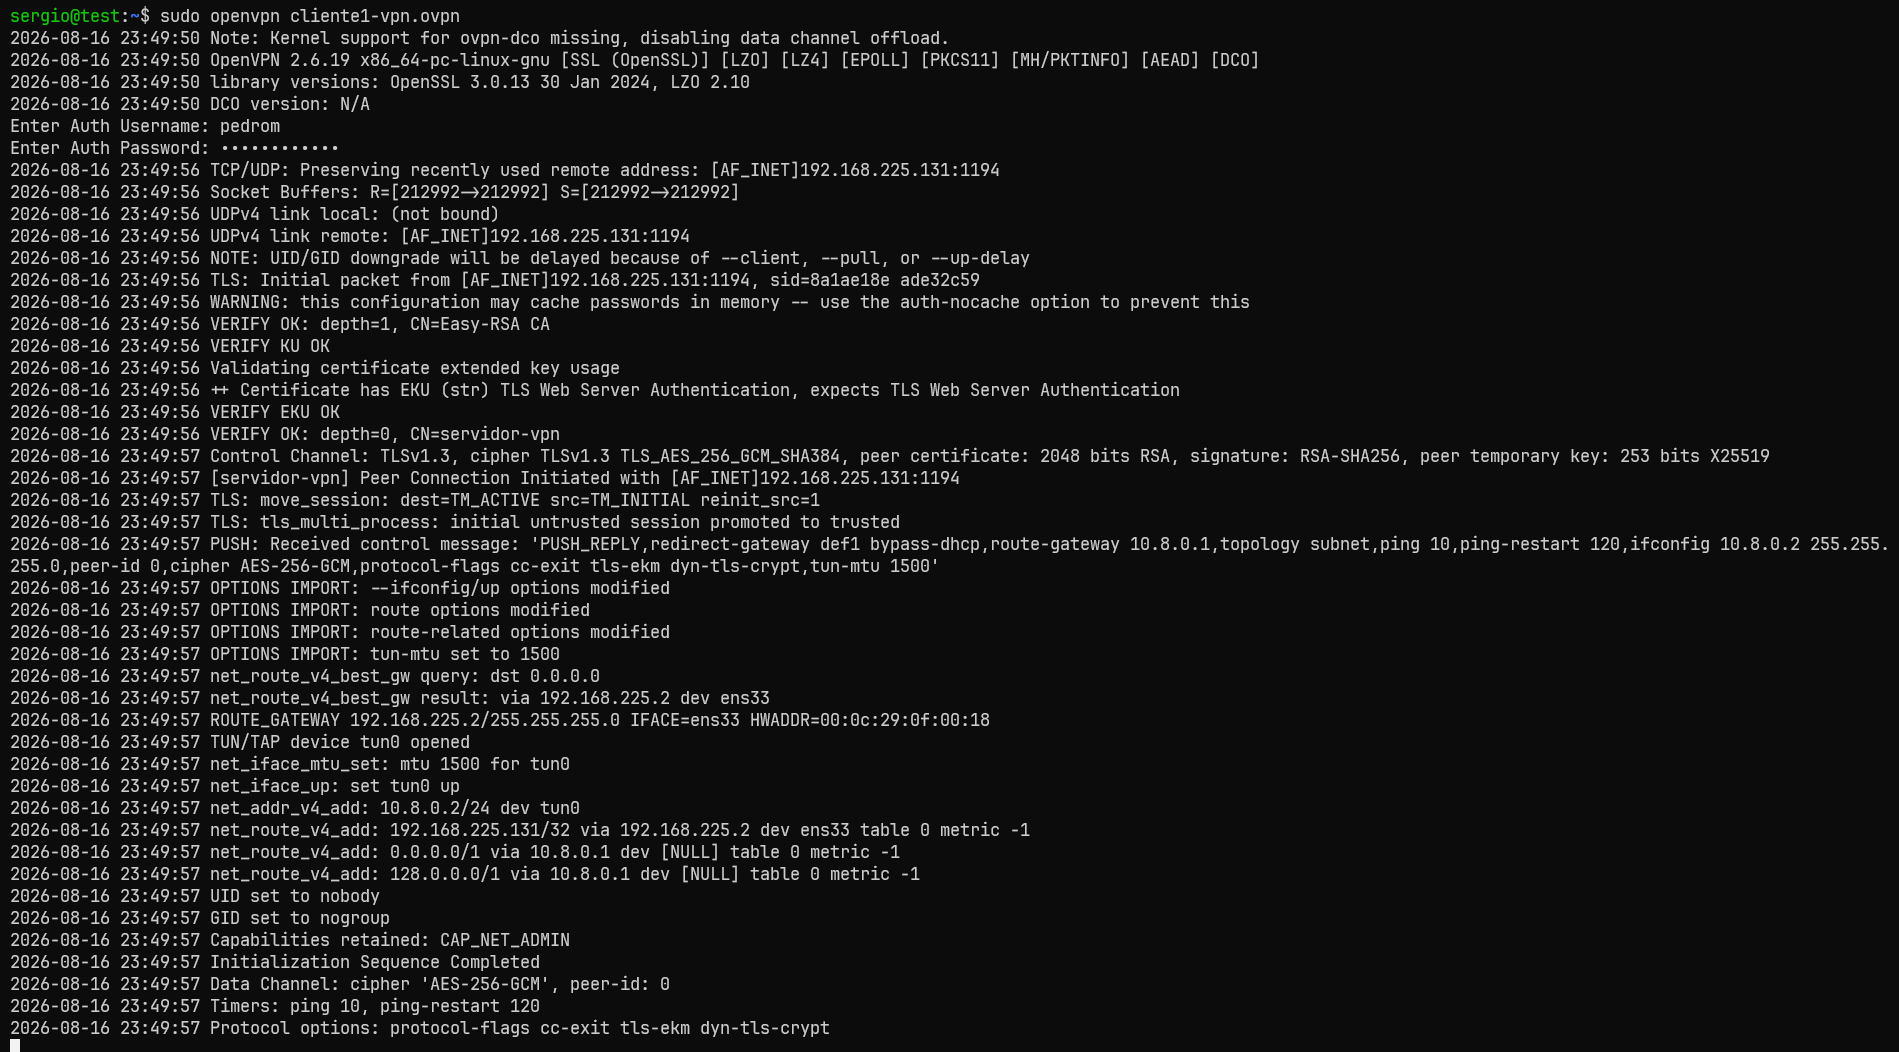
\includegraphics[width=0.85\textwidth]{imagenes/figuras/II-desarrollo-metodologico/pruebas/figura-6.png}
		      \caption{Acceso de la Cuenta 1 a OpenVPN y rechazo del acceso a los servicios no autorizados.}
		      \label{fig:figura-6}
	      \end{figure}

	\item \textbf{Validación del usuario autorizado para OpenProject:} Se utilizaron las credenciales de la cuenta 2 para realizar intentos de autenticación en OpenVPN, OpenProject y Xen Orchestra. En este caso, el acceso autorizado correspondió a OpenProject, mientras que los intentos realizados en los otros dos servicios permitieron comprobar la restricción de acceso. En la \autoref{fig:figura-7} se observan los resultados obtenidos.
	      \begin{figure}[H]
		      \centering
		      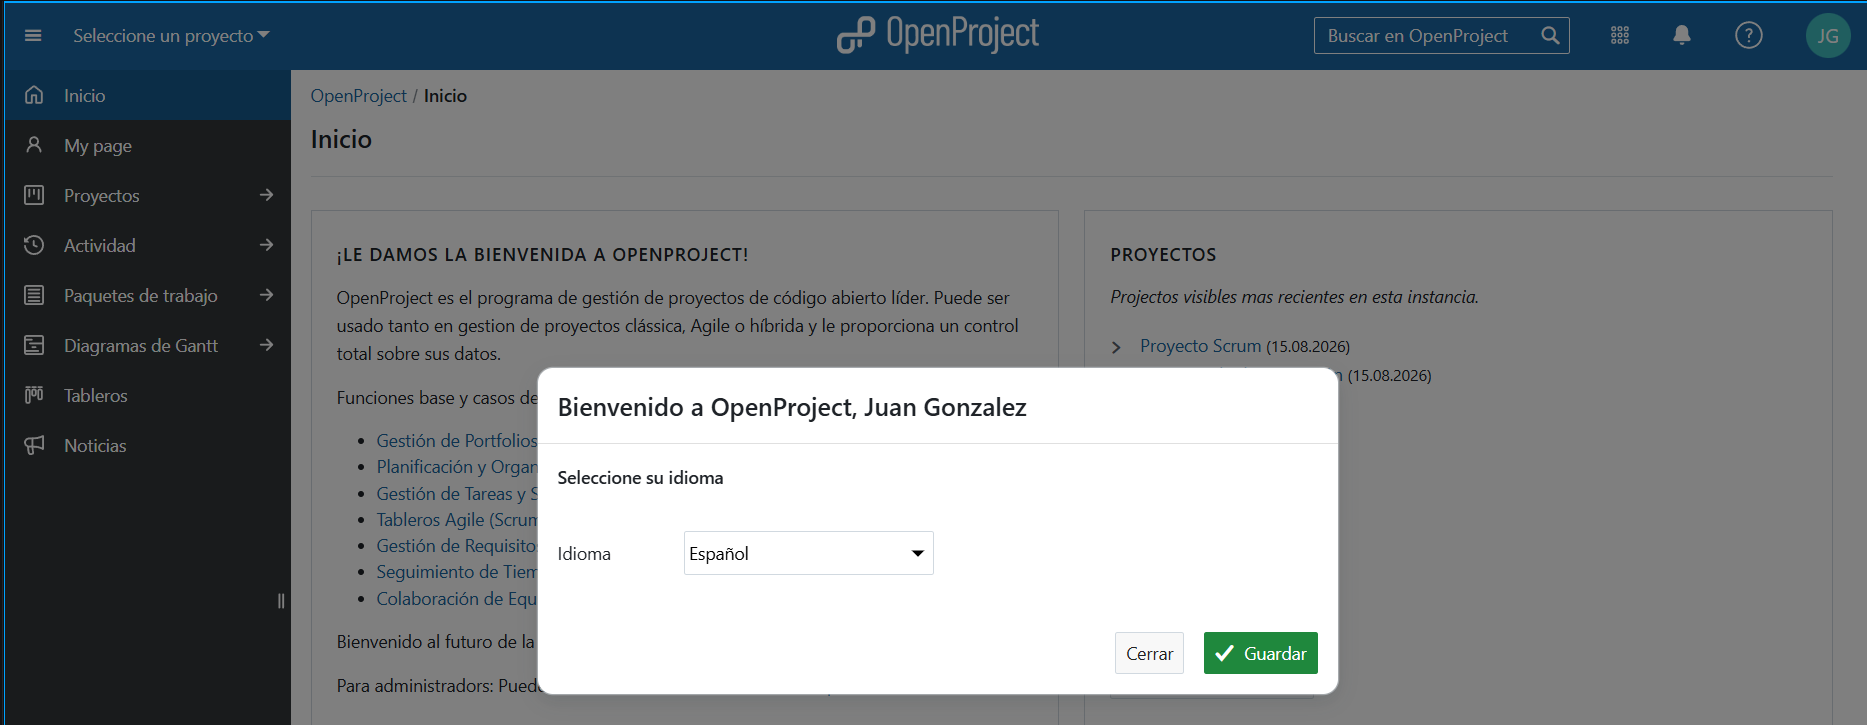
\includegraphics[width=0.85\textwidth]{imagenes/figuras/II-desarrollo-metodologico/pruebas/figura-7.png}
		      \caption{Acceso de la Cuenta 2 a OpenProject y rechazo del acceso a los servicios no autorizados.}
		      \label{fig:figura-7}
	      \end{figure}

	\item \textbf{Validación del usuario autorizado para Xen Orchestra:} Se utilizaron las credenciales de la cuenta 3 para realizar los intentos de autenticación en los tres servicios. El acceso a Xen Orchestra permitió comprobar la autorización correspondiente, mientras que los intentos realizados en OpenVPN y OpenProject permitieron verificar el rechazo de accesos no autorizados, tal como se presenta en la \autoref{fig:figura-8}.
	      \begin{figure}[H]
		      \centering
		      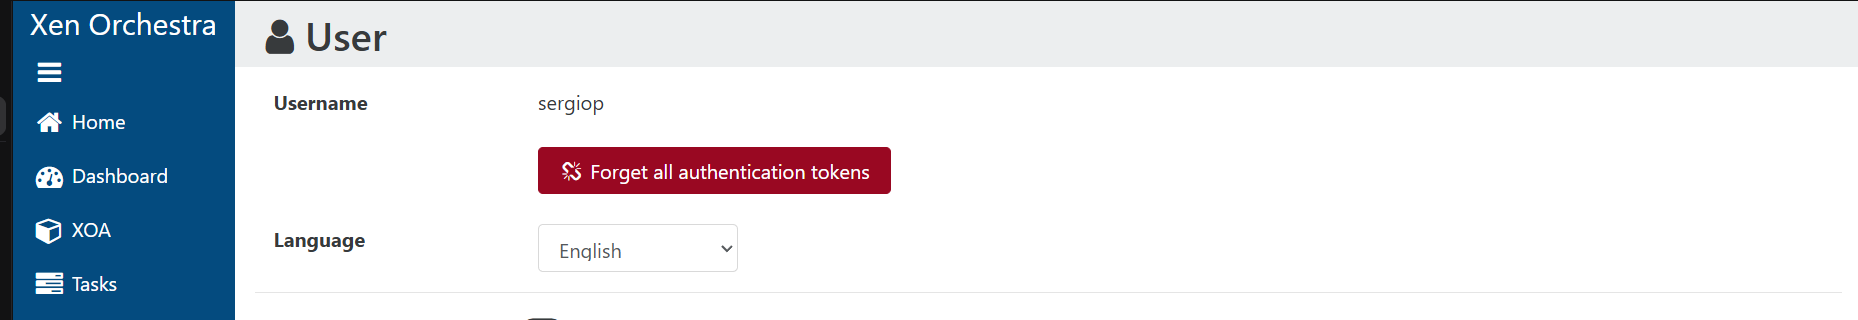
\includegraphics[width=0.85\textwidth]{imagenes/figuras/II-desarrollo-metodologico/pruebas/figura-8.png}
		      \caption{Acceso de la Cuenta 3 a Xen Orchestra y rechazo del acceso a los servicios no autorizados.}
		      \label{fig:figura-8}
	      \end{figure}

	\item \textbf{Consolidación de los resultados:} Finalmente, se consolidaron los resultados obtenidos durante los intentos de acceso de las tres cuentas para comparar el comportamiento de cada identidad frente a los servicios integrados, tal como se muestra en la \autoref{tab:pt02-consolidacion-resultados}.

	      \begingroup
	      \fontsize{8.5pt}{9.5pt}\selectfont
	      \renewcommand{\arraystretch}{1.3}
	      \setlength{\tabcolsep}{4pt}

	      \begin{longtable}{|
		      >{\raggedright\arraybackslash}p{2.5cm}|
		      >{\raggedright\arraybackslash}p{3.0cm}|
		      >{\raggedright\arraybackslash}p{2.5cm}|
		      >{\raggedright\arraybackslash}p{2.5cm}|
		      >{\raggedright\arraybackslash}p{3.0cm}|}

		      \caption{Consolidación de los resultados de acceso obtenidos en PT-02}
		      \label{tab:pt02-consolidacion-resultados}
		      \\
		      \hline
		      \rowcolor[gray]{0.85}
		      \textbf{Cuenta}      &
		      \textbf{Grupo}       &
		      \textbf{OpenVPN}     &
		      \textbf{OpenProject} &
		      \textbf{Xen Orchestra}
		      \\
		      \hline
		      \endfirsthead

		      \hline
		      \rowcolor[gray]{0.85}
		      \textbf{Cuenta}      &
		      \textbf{Grupo}       &
		      \textbf{OpenVPN}     &
		      \textbf{OpenProject} &
		      \textbf{Xen Orchestra}
		      \\
		      \hline
		      \endhead

		      Cuenta 1             & OpenVPN       & Permitido & Rechazado & Rechazado \\ \hline
		      Cuenta 2             & OpenProject   & Rechazado & Permitido & Rechazado \\ \hline
		      Cuenta 3             & Xen Orchestra & Rechazado & Rechazado & Permitido
	      \end{longtable}
	      \endgroup
	      \normalsize

	      Esta consolidación permitió comprobar que la autorización se mantuvo diferenciada entre los tres servicios a partir de la pertenencia de las cuentas a los grupos definidos en FreeIPA.
\end{enumerate}
\textbf{Estado:} Cumple.\\
\textbf{Observaciones:} La prueba permitió comprobar que la gestión centralizada de las identidades en FreeIPA puede complementarse con una autorización diferenciada para cada sistema integrado. La pertenencia a grupos permitió determinar los servicios a los cuales cada cuenta se encontraba autorizada, mientras que los intentos de acceso rechazados permitieron comprobar la aplicación efectiva de estas restricciones.
Los resultados aportaron evidencia para R-01, al demostrar la gestión centralizada de las identidades junto con una autorización diferenciada, y para R-04, al demostrar el control de los accesos mediante los permisos definidos en los grupos.

\subsection{PT-03 - Gestión del ciclo de vida de las cuentas}
\textbf{Requisito asociado:} R-02.\\
\textbf{Objetivo:} Verificar la capacidad del servicio de directorio para gestionar el ciclo de vida de las cuentas, considerando las operaciones de creación, actualización, habilitación, deshabilitación, revocación y expiración, así como el efecto de estos cambios sobre el acceso de los usuarios a los servicios integrados.\\
\textbf{Resultado esperado:} Las operaciones realizadas sobre la cuenta deben modificar correctamente su estado dentro del directorio y reflejarse en las condiciones de acceso a los servicios integrados.
Se espera que una cuenta creada pueda ser gestionada desde FreeIPA, que sus atributos puedan ser actualizados y que su estado determine la posibilidad de autenticación. Una cuenta habilitada debe poder acceder cuando cuenta con la autorización correspondiente, mientras que una cuenta deshabilitada o revocada debe tener restringido el acceso.\\
\textbf{Precondiciones:}
\begin{itemize}
	\item El servidor de FreeIPA se encuentra operativo.
	\item Los servicios integrados se encuentran disponibles.
	\item Se dispone de una cuenta de prueba destinada a validar las diferentes etapas del ciclo de vida.
	\item Las políticas y configuraciones necesarias para la gestión de cuentas se encuentran establecidas.
\end{itemize}
\textbf{Datos de prueba:} Se utilizó una cuenta de prueba gestionada desde FreeIPA. Sobre esta cuenta se realizaron las operaciones correspondientes a las diferentes etapas del ciclo de vida, verificando el estado de la identidad y su capacidad de acceso después de cada modificación.\\
\textbf{Procedimiento y evidencias:}
\begin{enumerate}
	\item \textbf{Creación de la cuenta:} Se creó una nueva cuenta de usuario en FreeIPA, proporcionando los atributos requeridos para su identificación y gestión. Una vez finalizada la creación, se verificó que la cuenta haya quedado registrada correctamente en el directorio, como se observa en la \autoref{fig:figura-9}.
	      \begin{figure}[H]
		      \centering
		      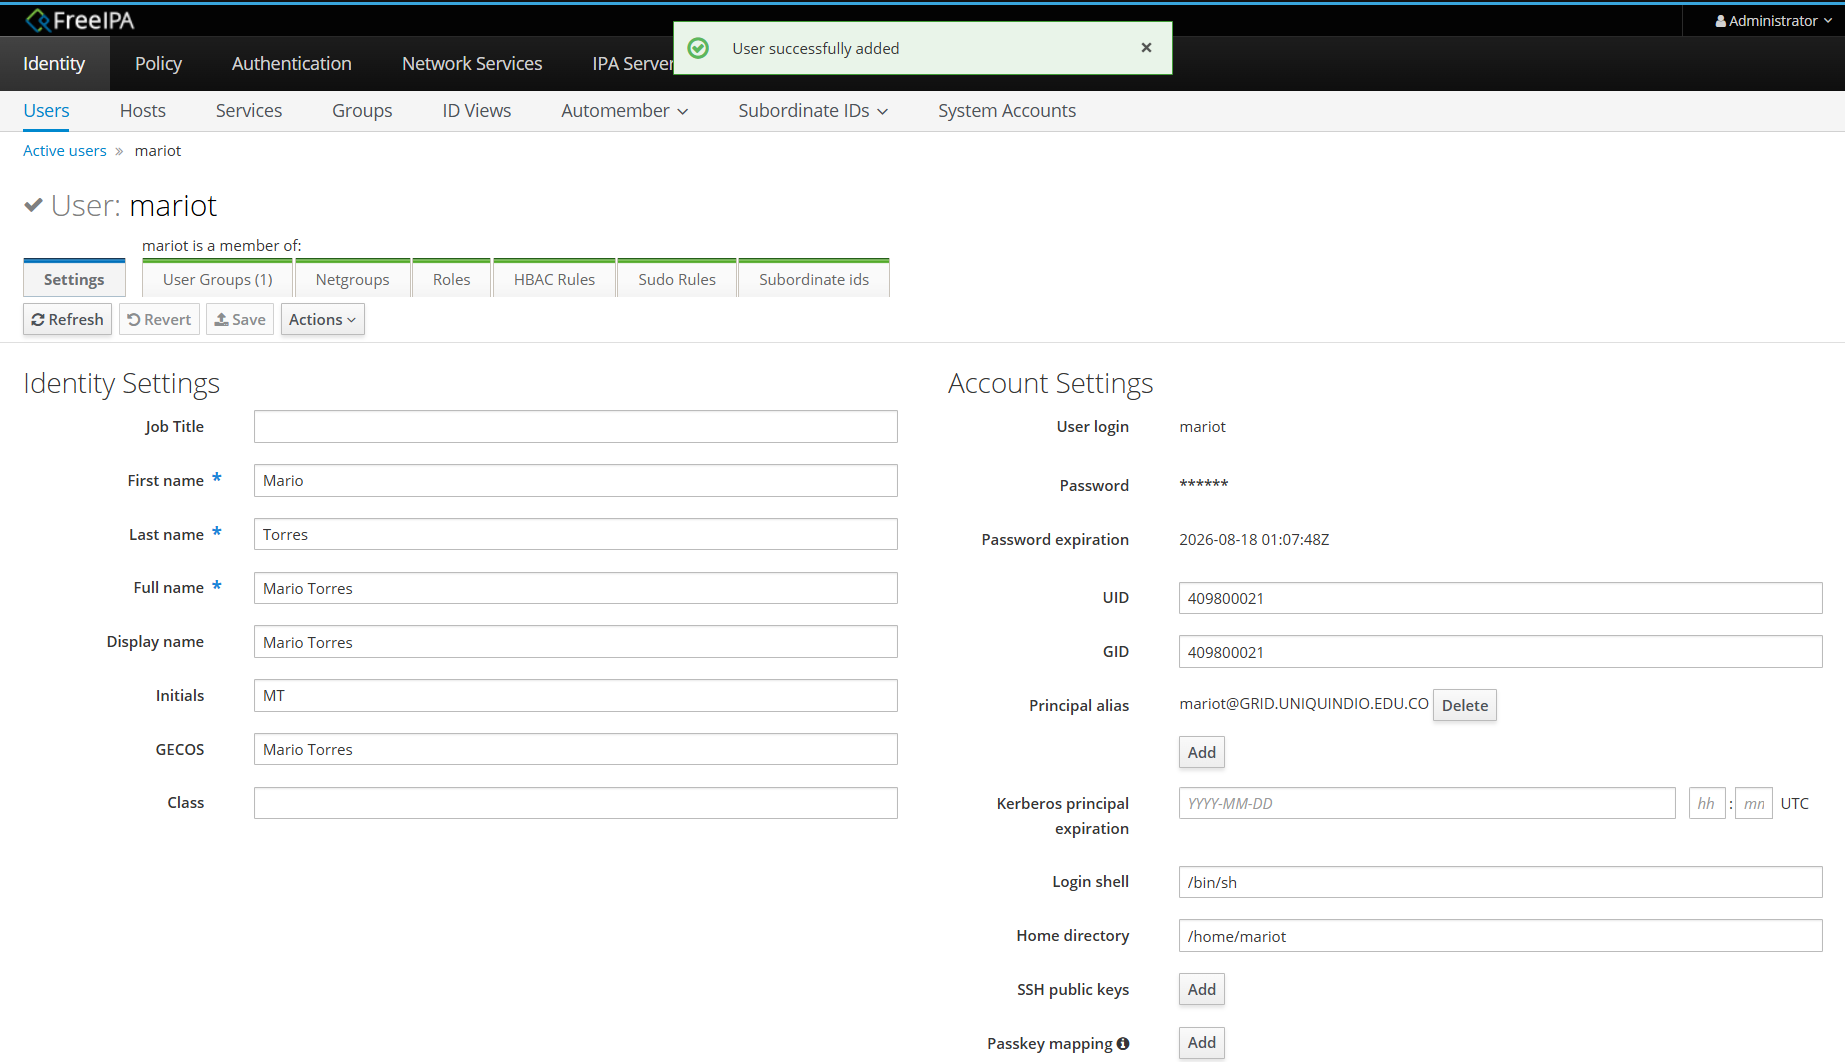
\includegraphics[width=0.85\textwidth]{imagenes/figuras/II-desarrollo-metodologico/pruebas/figura-9.png}
		      \caption{Creación y estado inicial de la cuenta de prueba en FreeIPA.}
		      \label{fig:figura-9}
	      \end{figure}

	\item \textbf{Actualización de la información de la cuenta:} Se modificaron los atributos definidos para la cuenta de prueba y se verificó posteriormente que los cambios fueran reflejados en la información almacenada en FreeIPA, tal como se muestra en la \autoref{fig:figura-10}.
	      \begin{figure}[H]
		      \centering
		      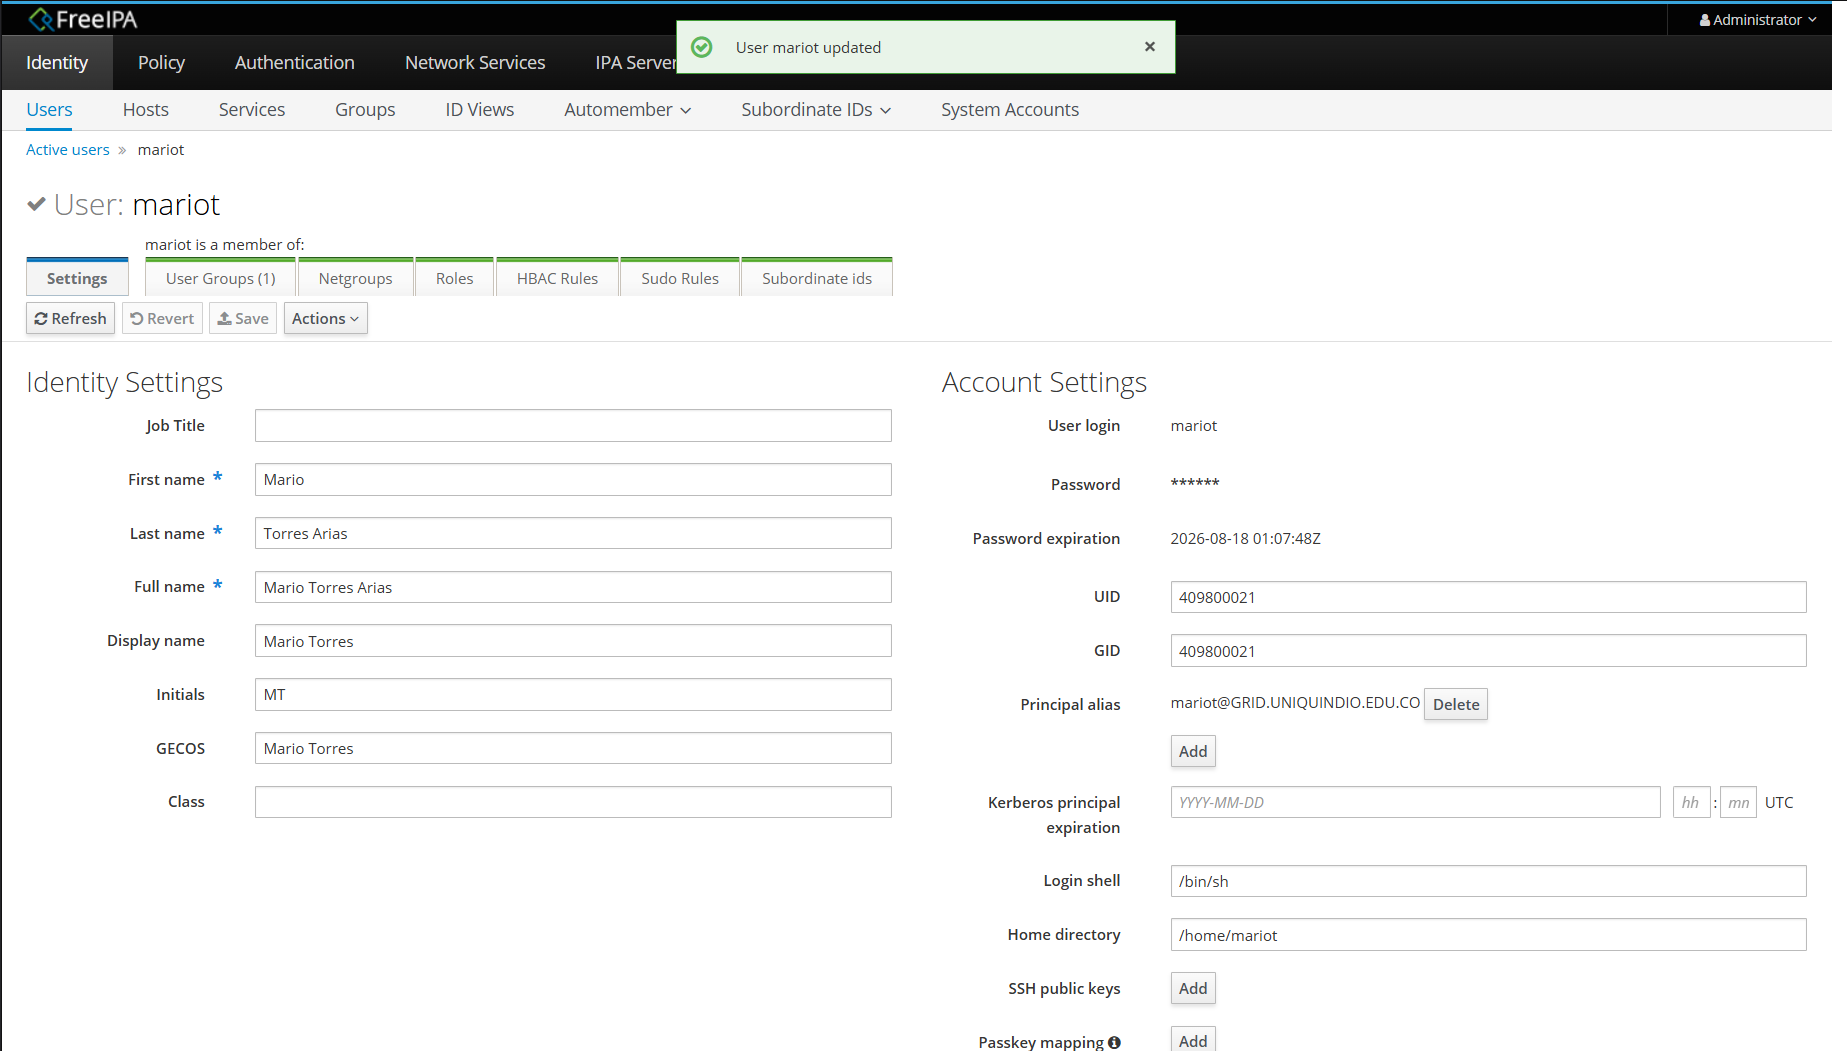
\includegraphics[width=0.85\textwidth]{imagenes/figuras/II-desarrollo-metodologico/pruebas/figura-10.png}
		      \caption{Actualización de los atributos de la cuenta de prueba en FreeIPA.}
		      \label{fig:figura-10}
	      \end{figure}

	\item \textbf{Habilitación de la cuenta y validación del acceso:} Se verificó que la cuenta se encontrará habilitada y con autorización de acceso a uno de los servicios, posteriormente se realizó un intento de autenticación en el servicio autorizado. El acceso se verificó utilizando las credenciales asociadas a la cuenta administrada por FreeIPA, como se presenta en la \autoref{fig:figura-11}.
	      \begin{figure}[H]
		      \centering
		      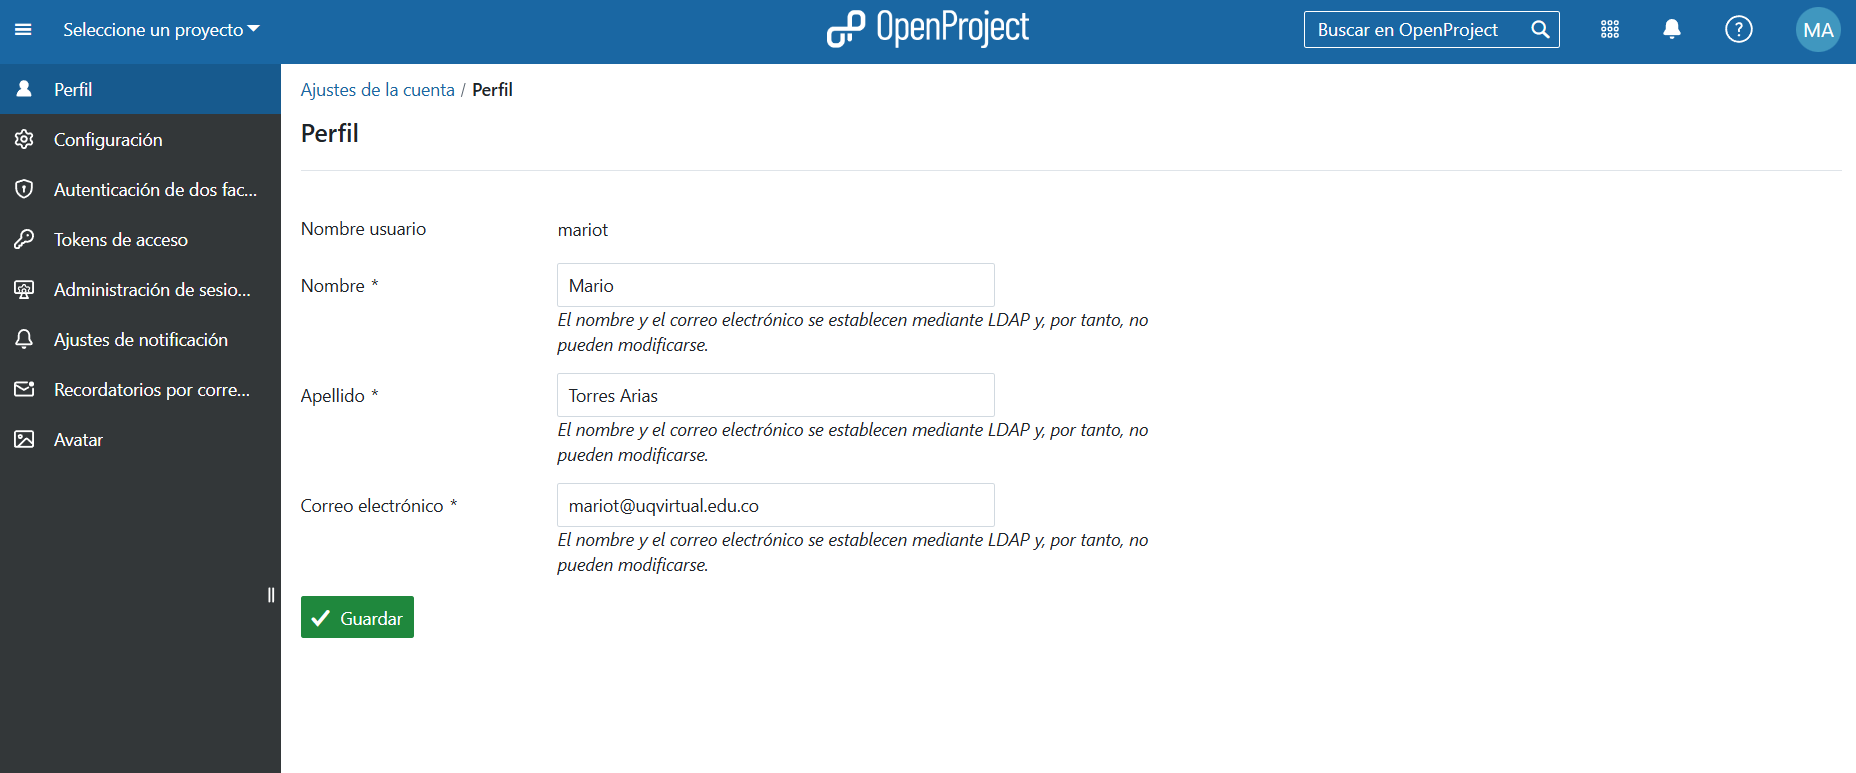
\includegraphics[width=0.85\textwidth]{imagenes/figuras/II-desarrollo-metodologico/pruebas/figura-11.png}
		      \caption{Estado habilitado de la cuenta y acceso autorizado al servicio integrado.}
		      \label{fig:figura-11}
	      \end{figure}

	\item \textbf{Deshabilitación de la cuenta y validación del acceso:} Se deshabilitó la cuenta desde FreeIPA, como se observa en la \autoref{fig:figura-12}, y posteriormente se realizó un nuevo intento de autenticación en el servicio utilizado en el paso anterior. El resultado obtenido se contrastó con el estado de la cuenta en el directorio, tal como se presenta en la \autoref{fig:figura-xx}.
	      \begin{figure}[H]
		      \centering
		      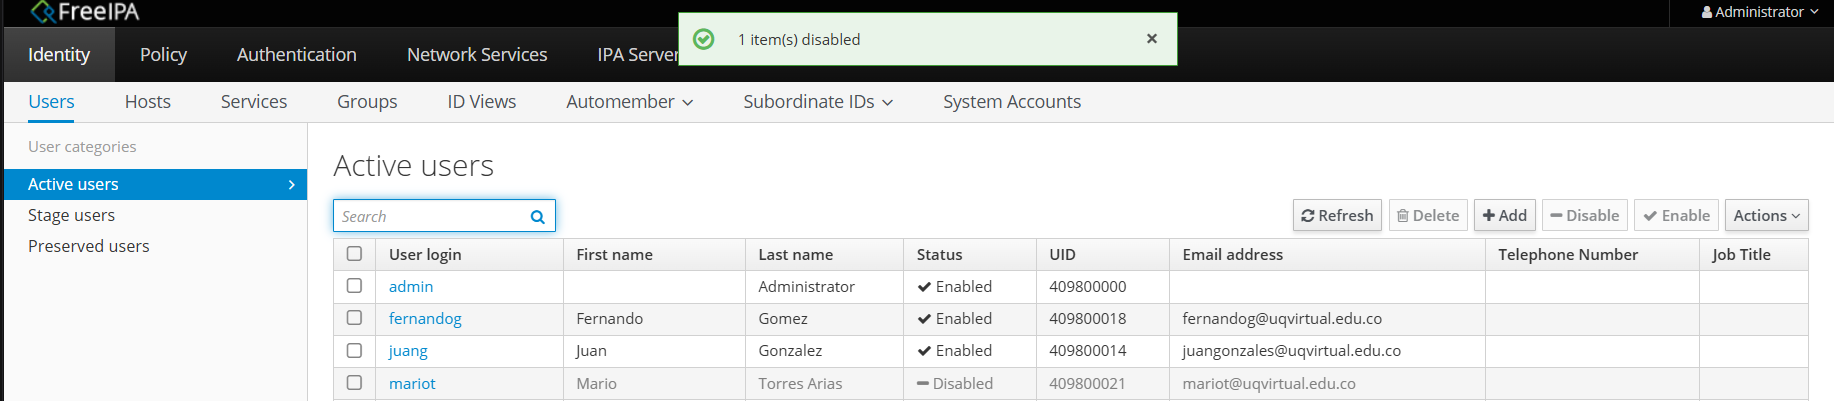
\includegraphics[width=0.85\textwidth]{imagenes/figuras/II-desarrollo-metodologico/pruebas/figura-12.png}
		      \caption{Cuenta deshabilitada en FreeIPA.}
		      \label{fig:figura-12}
	      \end{figure}

	      \begin{figure}[H]
		      \centering
		      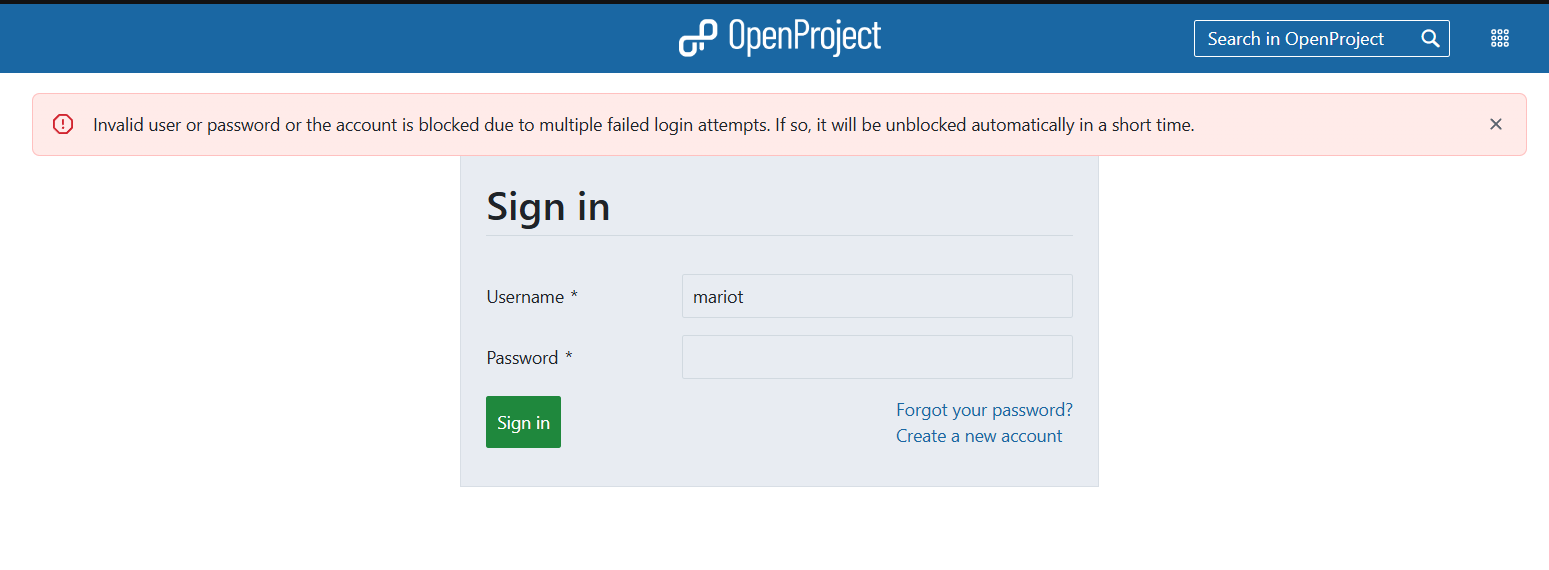
\includegraphics[width=0.85\textwidth]{imagenes/figuras/II-desarrollo-metodologico/pruebas/figura-xx.png}
		      \caption{Rechazo del acceso al servicio integrado tras la deshabilitación de la cuenta en FreeIPA}
		      \label{fig:figura-xx}
	      \end{figure}

	\item \textbf{Habilitación nuevamente de la cuenta:} Se habilitó nuevamente la cuenta en FreeIPA, como se muestra en la \autoref{fig:figura-13}, y se realizó un nuevo intento de acceso al servicio integrado, con el propósito de verificar si el cambio de estado permitía recuperar la capacidad de autenticación. El resultado se presenta en la \autoref{fig:figura-14}.
	      \begin{figure}[H]
		      \centering
		      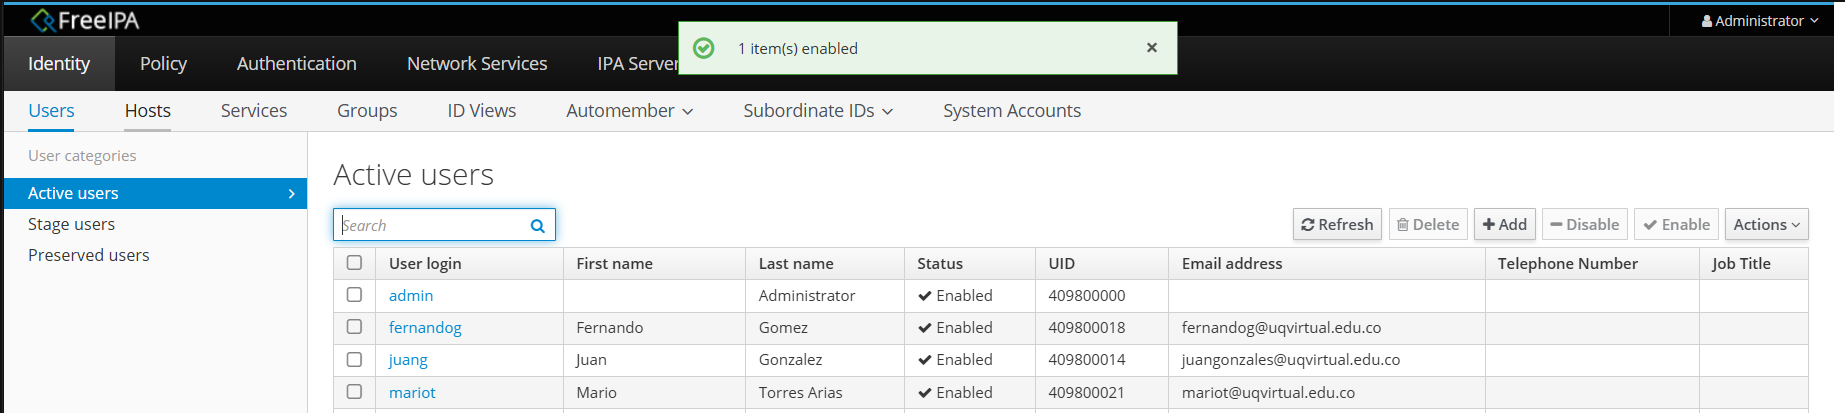
\includegraphics[width=0.85\textwidth]{imagenes/figuras/II-desarrollo-metodologico/pruebas/figura-13.png}
		      \caption{Habilitación de la cuenta de prueba en FreeIPA}
		      \label{fig:figura-13}
	      \end{figure}

	      \begin{figure}[H]
		      \centering
		      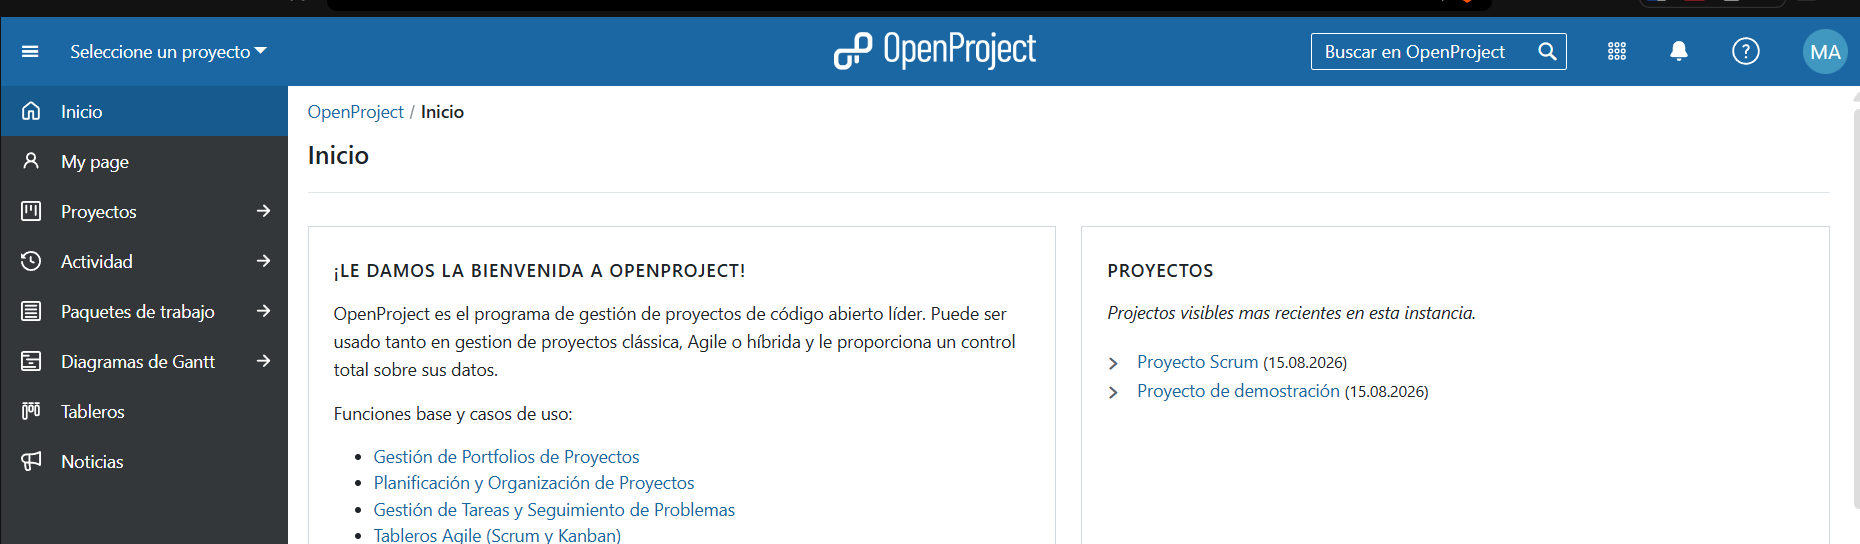
\includegraphics[width=0.85\textwidth]{imagenes/figuras/II-desarrollo-metodologico/pruebas/figura-14.png}
		      \caption{Recuperación del acceso al servicio integrado tras la habilitación de la cuenta en FreeIPA}
		      \label{fig:figura-14}
	      \end{figure}

	\item \textbf{Eliminación de la cuenta:} Se realizó la eliminación de la cuenta de forma preservada, como se observa en la \autoref{fig:figura-15}. Posteriormente, se verificó el estado resultante de la identidad y se realizó un intento de autenticación para comprobar el efecto de la revocación sobre el acceso, tal como se presenta en la \autoref{fig:figura-16}.
	      \begin{figure}[H]
		      \centering
		      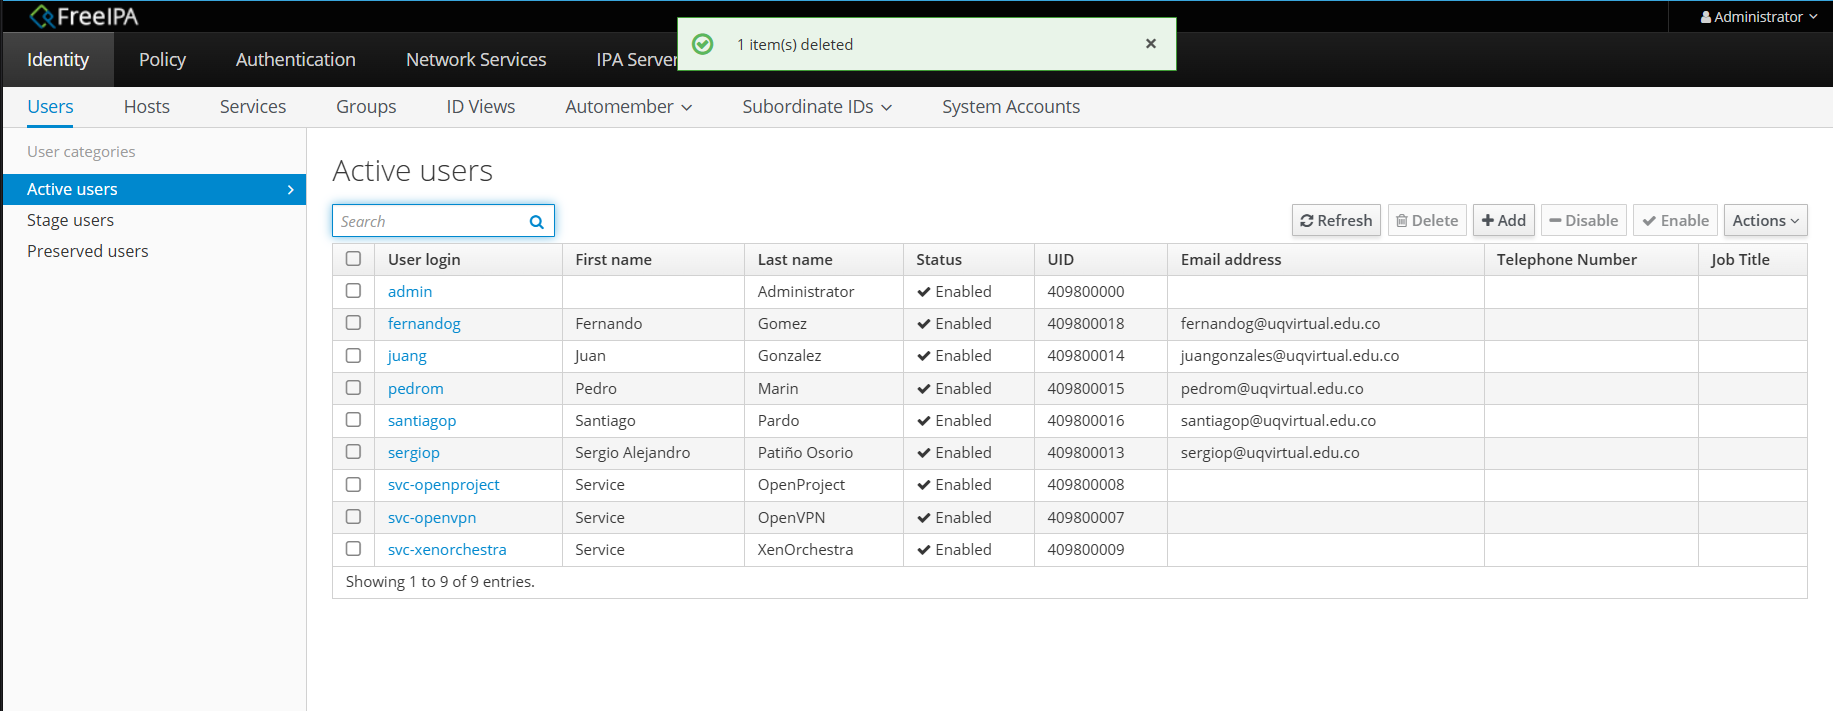
\includegraphics[width=0.85\textwidth]{imagenes/figuras/II-desarrollo-metodologico/pruebas/figura-15.png}
		      \caption{Revocación de la cuenta de prueba.}
		      \label{fig:figura-15}
	      \end{figure}

	      \begin{figure}[H]
		      \centering
		      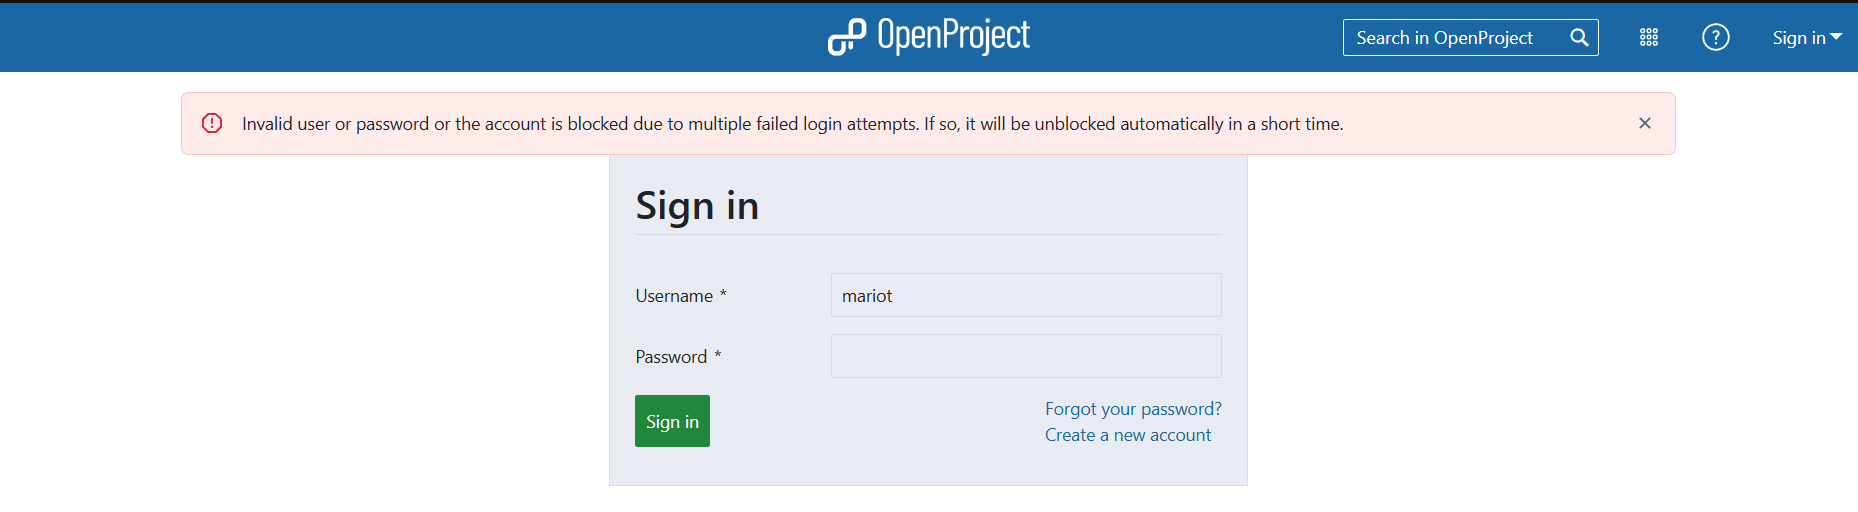
\includegraphics[width=0.85\textwidth]{imagenes/figuras/II-desarrollo-metodologico/pruebas/figura-16.png}
		      \caption{Rechazo del acceso al servicio integrado tras la revocación de la cuenta de prueba}
		      \label{fig:figura-16}
	      \end{figure}
\end{enumerate}
\textbf{Estado:} Cumple.\\
\textbf{Observaciones:} La prueba permite verificar el comportamiento de las operaciones de gestión del ciclo de vida de las cuentas y su relación con el acceso a los servicios integrados. Las evidencias obtenidas durante cada etapa permitieron establecer una relación directa entre los cambios realizados sobre la identidad en FreeIPA y el comportamiento observado en el servicio utilizado para la validación.

\subsection{PT-04 - Aplicación de políticas de seguridad y credenciales}
\textbf{Requisitos asociados:} R-03, R-06.\\
\textbf{Objetivo:} Verificar la definición y aplicación de las políticas de seguridad para usuarios y credenciales configuradas en FreeIPA, comprobando su efecto sobre las contraseñas y sobre los mecanismos de autenticación utilizados por los usuarios.\\
\textbf{Resultado esperado:} Las contraseñas que no cumplan las condiciones definidas en las políticas de seguridad deben ser rechazadas por FreeIPA, mientras que una contraseña que cumpla los requisitos establecidos debe poder ser utilizada para la autenticación.
Asimismo, ante la realización de intentos consecutivos de autenticación incorrectos, el comportamiento de la cuenta debe corresponder con los parámetros de bloqueo configurados en la política.\\
\textbf{Precondiciones:}
\begin{itemize}
	\item El servidor de FreeIPA se encuentra operativo.
	\item Las políticas de contraseñas se encuentran configuradas.
	\item Se dispone de una cuenta de prueba.
	\item La cuenta de prueba se encuentra habilitada.
	\item Los servicios integrados se encuentran disponibles para realizar las validaciones de autenticación.
\end{itemize}
\textbf{Datos de prueba:} Se utilizó una cuenta de prueba gestionada en FreeIPA y se realizaron operaciones relacionadas con sus credenciales para comprobar la aplicación de las políticas configuradas.\\
\textbf{Procedimiento y evidencias:}
\begin{enumerate}
	\item \textbf{Verificación de las políticas configuradas:} Se consultó la configuración de las políticas de contraseñas establecidas en FreeIPA, verificando los parámetros definidos para las credenciales de los usuarios, como se presenta en la \autoref{fig:figura-17}.
	      \begin{figure}[H]
		      \centering
		      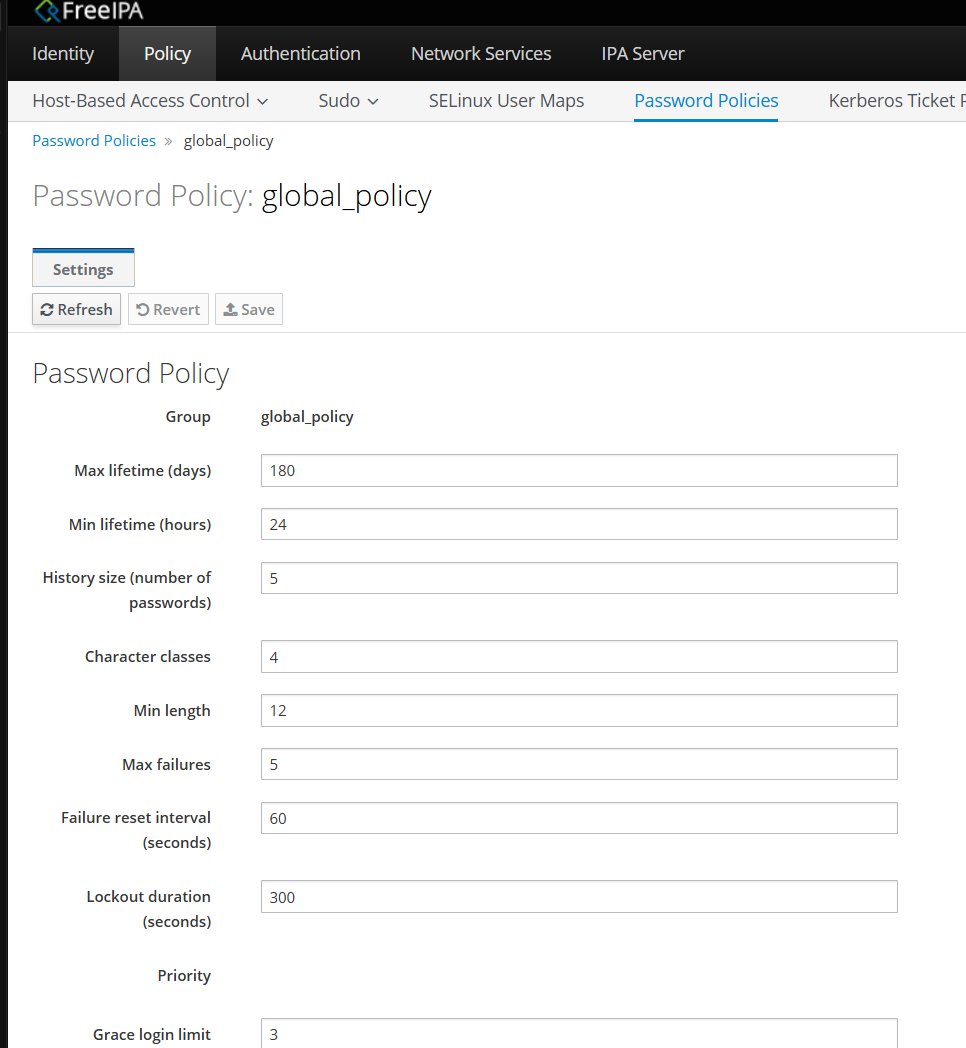
\includegraphics[width=0.85\textwidth]{imagenes/figuras/II-desarrollo-metodologico/pruebas/figura-17.png}
		      \caption{Políticas de contraseñas configuradas en FreeIPA.}
		      \label{fig:figura-17}
	      \end{figure}

	\item \textbf{Validación de la longitud mínima de la contraseña:} Se intentó establecer para la cuenta de prueba una contraseña que no cumpliera con la longitud mínima definida en la política. Posteriormente, se verificó la respuesta de FreeIPA ante el intento de establecer la credencial, tal como se observa en la \autoref{fig:figura-18}. El rechazo permitió comprobar que la política configurada se aplicó durante la modificación de las credenciales.
	      \begin{figure}[H]
		      \centering
		      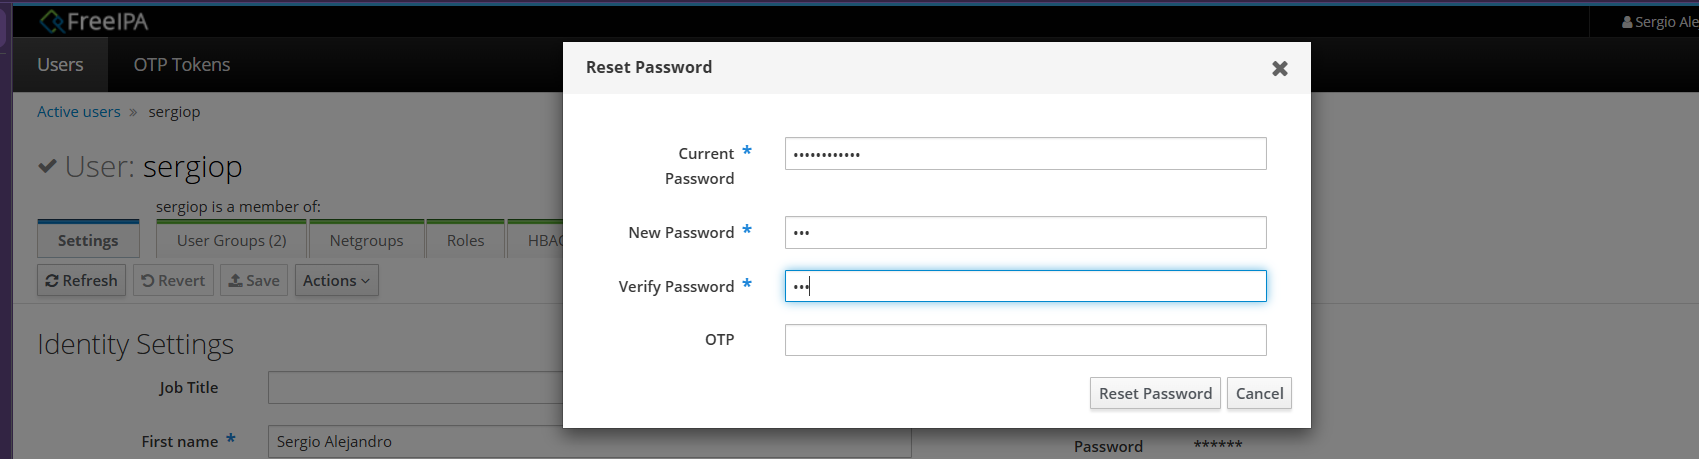
\includegraphics[width=0.85\textwidth]{imagenes/figuras/II-desarrollo-metodologico/pruebas/figura-18.png}
		      \caption{Rechazo de una contraseña que no cumple la longitud mínima establecida.}
		      \label{fig:figura-18}
	      \end{figure}

	\item \textbf{Validación de los requisitos de complejidad:} Se realizó un intento de establecer una contraseña que no cumpliera con los requisitos de complejidad definidos en la política. Se verificó la respuesta generada por FreeIPA ante la credencial que no cumplía las condiciones establecidas, como se presenta en la \autoref{fig:figura-19}.
	      \begin{figure}[H]
		      \centering
		      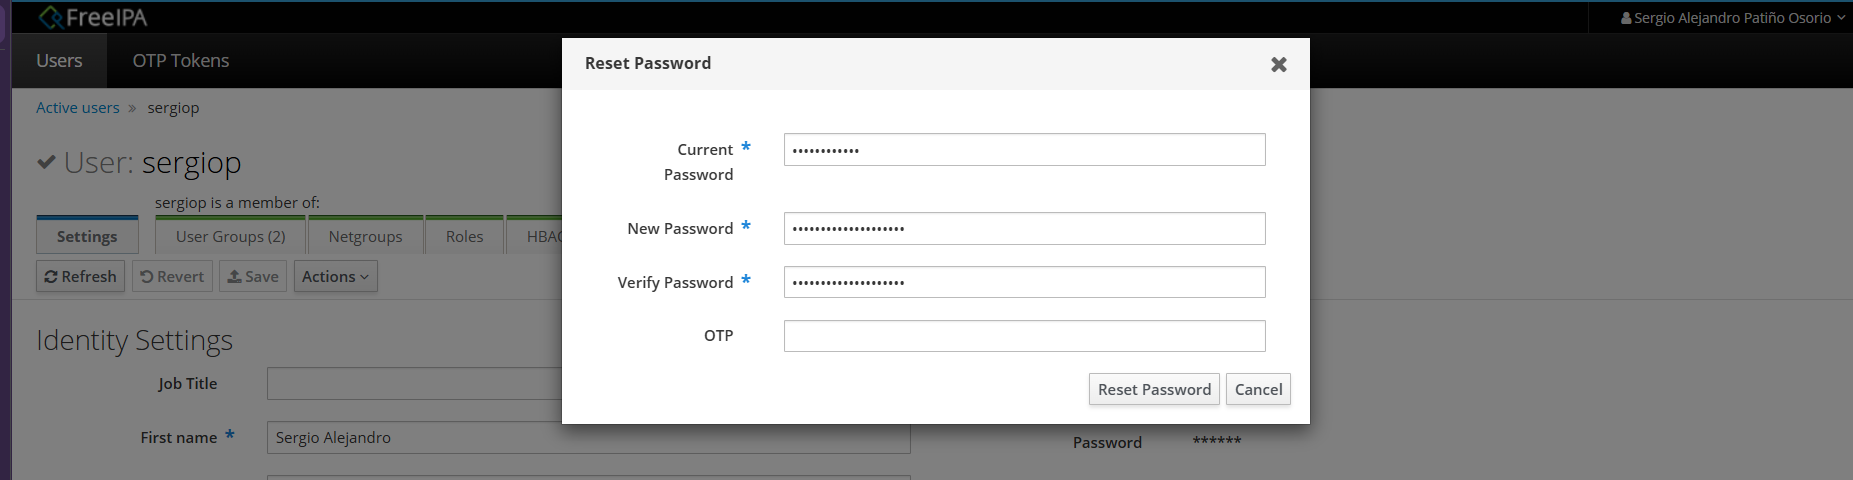
\includegraphics[width=0.85\textwidth]{imagenes/figuras/II-desarrollo-metodologico/pruebas/figura-19.png}
		      \caption{Rechazo de una contraseña que no cumple los requisitos de complejidad.}
		      \label{fig:figura-19}
	      \end{figure}

	\item \textbf{Validación de la contraseña que cumple las políticas:} Se estableció una contraseña que cumplía las condiciones definidas por la política de credenciales. Posteriormente, se realizó un intento de autenticación utilizando la nueva contraseña, tal como se muestra en la \autoref{fig:figura-20}.
	      \begin{figure}[H]
		      \centering
		      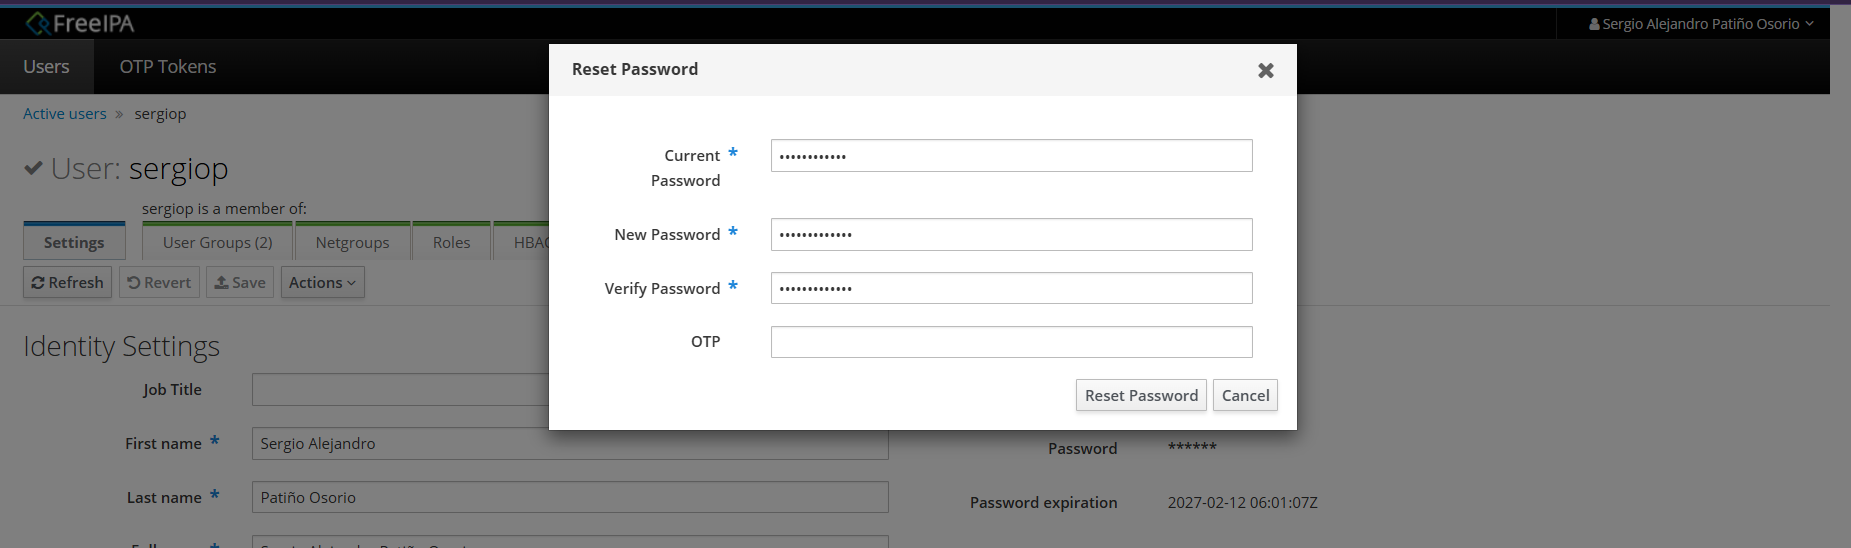
\includegraphics[width=0.85\textwidth]{imagenes/figuras/II-desarrollo-metodologico/pruebas/figura-20.png}
		      \caption{Establecimiento de una contraseña que cumple las políticas y autenticación exitosa.}
		      \label{fig:figura-20}
	      \end{figure}

	\item \textbf{Validación del control ante intentos de autenticación fallidos:} Se realizaron intentos consecutivos de autenticación utilizando credenciales incorrectas, con el propósito de verificar el comportamiento definido para los intentos fallidos y el bloqueo de la cuenta. Los resultados se observan en la \autoref{fig:figura-21}.
	      \begin{figure}[H]
		      \centering
		      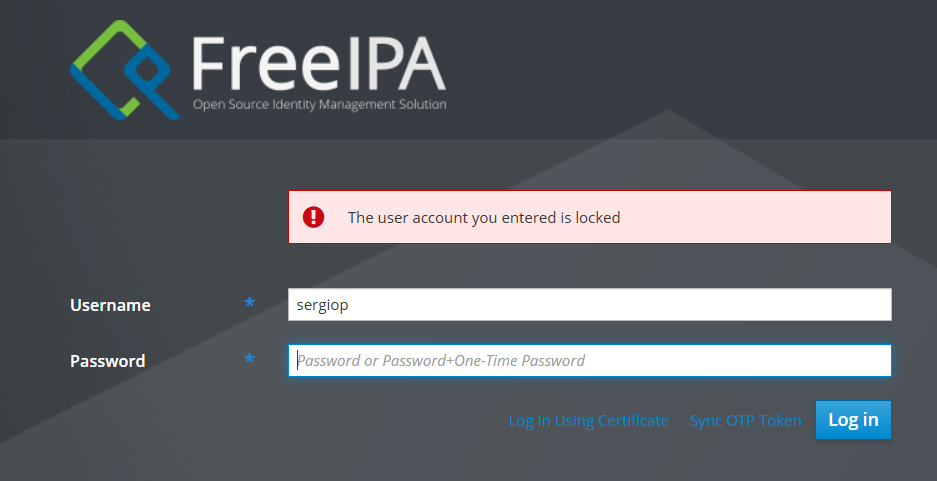
\includegraphics[width=0.85\textwidth]{imagenes/figuras/II-desarrollo-metodologico/pruebas/figura-21.png}
		      \caption{Aplicación de la política ante intentos consecutivos de autenticación fallidos.}
		      \label{fig:figura-21}
	      \end{figure}
\end{enumerate}
\textbf{Estado:} Cumple.\\
\textbf{Observaciones:} La prueba permite demostrar directamente la aplicación de las políticas de seguridad y credenciales correspondientes a R-03. Para R-06, sin embargo, es importante distinguir entre la aplicación de políticas de credenciales y la existencia de mecanismos adicionales de autenticación.

\subsection{PT-05 - Registro y trazabilidad de actividades}
\textbf{Requisito asociado:} R-05.\\
\textbf{Objetivo:} Verificar que las actividades relevantes relacionadas con la gestión de identidades y accesos queden registradas en los mecanismos de auditoría disponibles en FreeIPA, de manera que sea posible identificar la actividad realizada y consultar información que permita su posterior revisión.\\
\textbf{Resultado esperado:} Las actividades relevantes de gestión de identidades y accesos realizadas durante la prueba deben generar registros consultables en los mecanismos de auditoría disponibles en FreeIPA.
La información registrada debe permitir relacionar el evento con la actividad realizada y proporcionar datos suficientes para facilitar su revisión posterior.\\
\textbf{Precondiciones:}
\begin{itemize}
	\item El servidor de FreeIPA se encuentra operativo.
	\item Los mecanismos de registro y auditoría de FreeIPA se encuentran disponibles.
	\item Se dispone de una cuenta de prueba.
	\item Se cuenta con acceso administrativo suficiente para consultar los registros generados.
	\item Se dispone de una actividad de gestión de identidad que pueda ser utilizada para generar un evento de auditoría.
\end{itemize}
\textbf{Procedimiento y evidencias:}
\begin{enumerate}
	\item \textbf{Identificación de los mecanismos de registro:} Se consultaron los mecanismos de registro disponibles en el servidor de FreeIPA con el propósito de identificar los registros relacionados con las actividades de autenticación y administración de identidades, como se presenta en la \autoref{fig:figura-22}.
	      \begin{figure}[H]
		      \centering
		      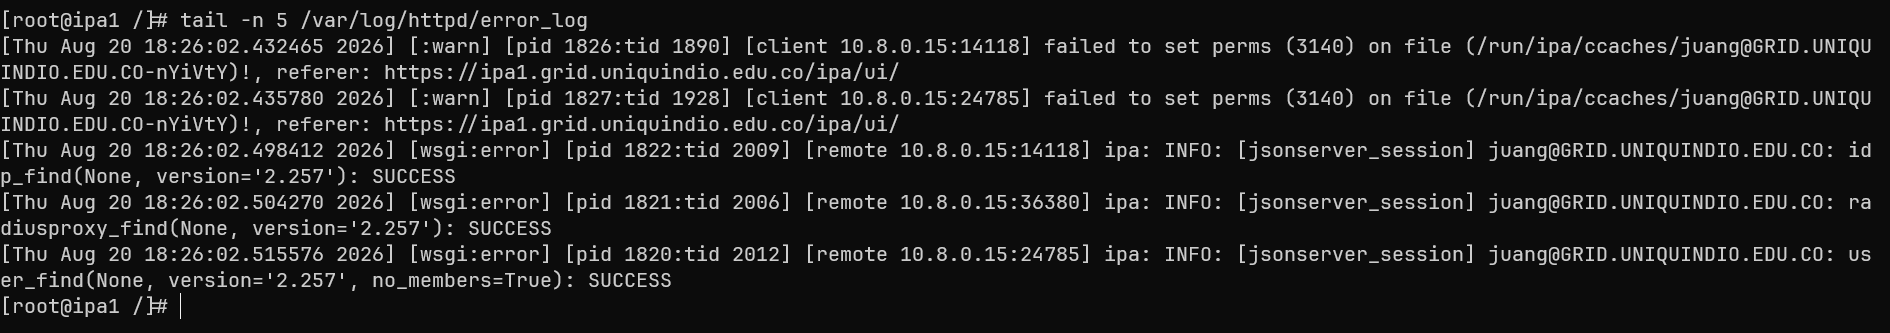
\includegraphics[width=0.85\textwidth]{imagenes/figuras/II-desarrollo-metodologico/pruebas/figura-22.png}
		      \caption{Registros de FreeIPA utilizados para la consulta de actividades de gestión de identidades y accesos.}
		      \label{fig:figura-22}
	      \end{figure}

	\item \textbf{Generación de una actividad de gestión de identidad:} Se realizó una operación sobre la cuenta de prueba desde FreeIPA, utilizando una actividad previamente definida para la validación, como se observa en la \autoref{fig:figura-23}. La operación se ejecutó de manera controlada con el propósito de posteriormente localizar el evento correspondiente en los registros.
	      \begin{figure}[H]
		      \centering
		      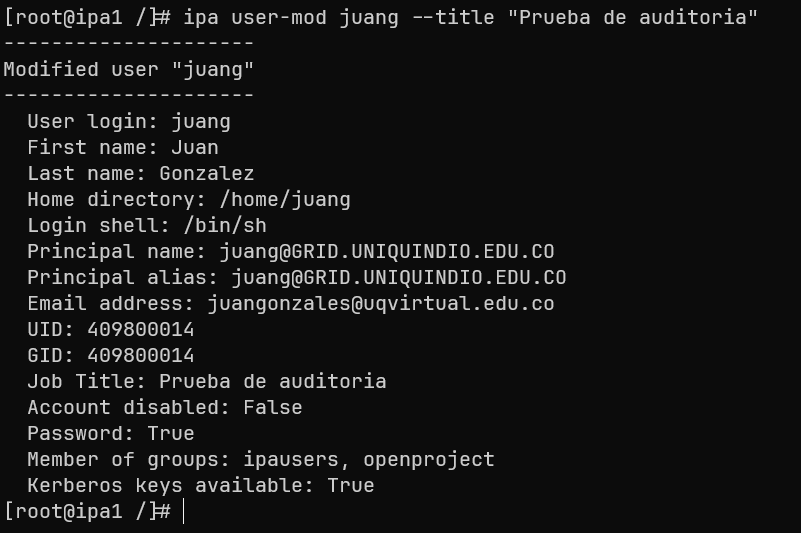
\includegraphics[width=0.85\textwidth]{imagenes/figuras/II-desarrollo-metodologico/pruebas/figura-23.png}
		      \caption{Actividad de gestión de identidad realizada sobre la cuenta de prueba.}
		      \label{fig:figura-23}
	      \end{figure}

	\item \textbf{Consulta del registro generado:} Una vez realizada la operación, se consultaron los registros correspondientes en el servidor para localizar la actividad generada, tal como se presenta en la \autoref{fig:figura-24}. Se verificó la información disponible en el evento registrado y su correspondencia con la operación realizada sobre la cuenta de prueba.
	      \begin{figure}[H]
		      \centering
		      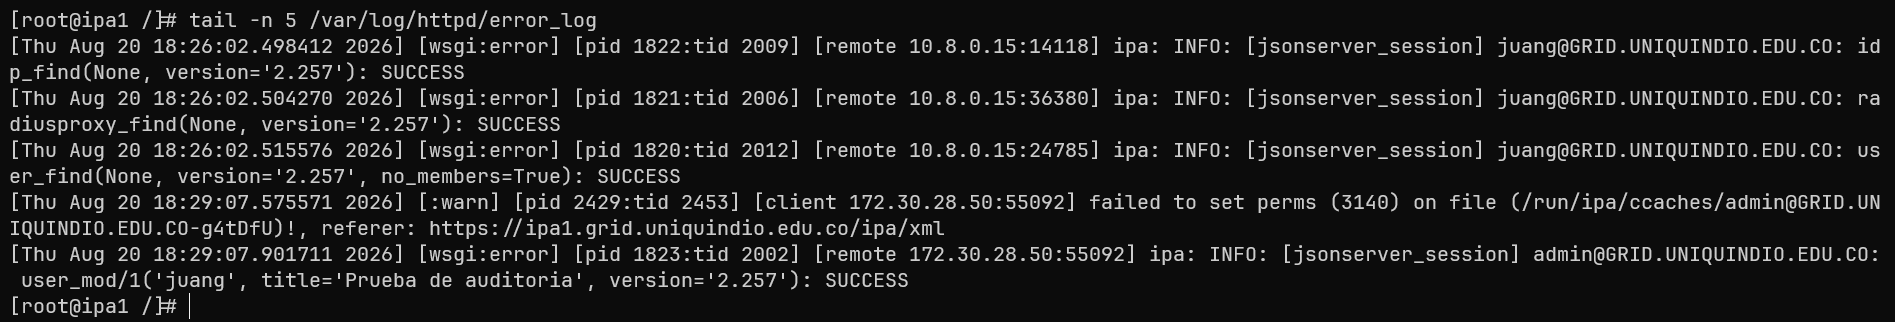
\includegraphics[width=0.85\textwidth]{imagenes/figuras/II-desarrollo-metodologico/pruebas/figura-24.png}
		      \caption{Registro de la actividad de gestión realizada sobre la cuenta de prueba.}
		      \label{fig:figura-24}
	      \end{figure}

	\item \textbf{Validación de la trazabilidad:} Se contrastó la información registrada con la actividad realizada durante la prueba, verificando que los datos disponibles permitieran relacionar el evento registrado con la operación efectuada sobre la identidad. Los resultados de esta validación se presentan en la \autoref{tab:pt05-trazabilidad}.

	      \begingroup
	      \fontsize{8.5pt}{9.5pt}\selectfont
	      \renewcommand{\arraystretch}{1.3}
	      \setlength{\tabcolsep}{4pt}

	      \begin{longtable}{|
		      >{\raggedright\arraybackslash}p{3.0cm}|
		      >{\raggedright\arraybackslash}p{3.5cm}|
		      >{\raggedright\arraybackslash}p{4.5cm}|
		      >{\raggedright\arraybackslash}p{2.5cm}|}

		      \caption{Validación de la trazabilidad de eventos de auditoría}
		      \label{tab:pt05-trazabilidad}
		      \\
		      \hline
		      \rowcolor[gray]{0.85}
		      \textbf{Elemento a verificar}      &
		      \textbf{Actividad realizada}       &
		      \textbf{Información registrada}    &
		      \textbf{Correspondencia}
		      \\
		      \hline
		      \endfirsthead

		      \caption{Validación de la trazabilidad de eventos de auditoría (continuación)}
		      \\
		      \hline
		      \rowcolor[gray]{0.85}
		      \textbf{Elemento a verificar}      &
		      \textbf{Actividad realizada}       &
		      \textbf{Información registrada}    &
		      \textbf{Correspondencia}
		      \\
		      \hline
		      \endhead

		      Identidad que ejecutó la operación & admin@\acs{GRID}.UNIQUINDIO.EDU.CO & admin@\acs{GRID}.UNIQUINDIO.EDU.CO & Sí \\ \hline
		      Operación                          & user mod                           & Modificación de usuario            & Sí \\ \hline
		      Identidad afectada                 & juang                              & juang                              & Sí \\ \hline
		      Atributo modificado                & title                              & title 'Prueba de auditoria'        & Sí \\ \hline
		      Resultado                          & Operación exitosa                  & SUCCESS                            & Sí \\ \hline
		      Fecha y hora                       & 20 de agosto de 2026, 18:29        & Thu Aug 20 18:29:07.901711 2026    & Sí \\ \hline
	      \end{longtable}
	      \endgroup
	      \normalsize
\end{enumerate}
\textbf{Estado:} Cumple.\\
\textbf{Observaciones:} La prueba permitió verificar la existencia de mecanismos de registro asociados a las actividades de gestión de identidades y accesos. Los registros obtenidos proporcionaron evidencia para determinar la capacidad de FreeIPA para mantener información susceptible de ser utilizada en procesos de revisión y auditoría, en correspondencia con el requisito R-05.

\subsection{PT-06 - Revisión de permisos y control de acceso}
\textbf{Requisito asociado:} R-04.\\
\textbf{Objetivo:} Verificar que sea posible consultar los grupos que autorizan el acceso a los servicios, permitiendo identificar qué usuarios están autorizados para acceder a cada uno de los servicios integrados.\\
\textbf{Resultado esperado:} La información disponible en FreeIPA debe permitir identificar los grupos utilizados para controlar el acceso y los usuarios pertenecientes a cada uno de ellos. A partir de esta información debe ser posible revisar los permisos asignados a las cuentas y determinar los servicios para los cuales se encuentran autorizadas.\\
\textbf{Precondiciones:}
\begin{itemize}
	\item El servidor de FreeIPA se encuentra operativo.
	\item Las cuentas de prueba se encuentran registradas y habilitadas.
	\item Los grupos de autorización utilizados para OpenVPN, OpenProject y Xen Orchestra se encuentran configurados.
	\item Las integraciones de los servicios con FreeIPA se encuentran operativas.
\end{itemize}
\textbf{Datos de prueba:} Se utilizaron las cuentas y grupos empleados durante PT-02, debido a que estos representan las autorizaciones establecidas para cada servicio. La información de pertenencia a grupos se utilizó para revisar los permisos asignados a los usuarios.\\
\textbf{Procedimiento y evidencia:}
\begin{enumerate}
	\item \textbf{Consulta de los grupos de autorización:} Se consultaron en FreeIPA los grupos utilizados para controlar el acceso a OpenVPN, OpenProject y Xen Orchestra. Se verificó la existencia de los grupos que permiten el acceso a los servicios integrados, como se muestra en la \autoref{fig:figura-25}.
	      \begin{figure}[H]
		      \centering
		      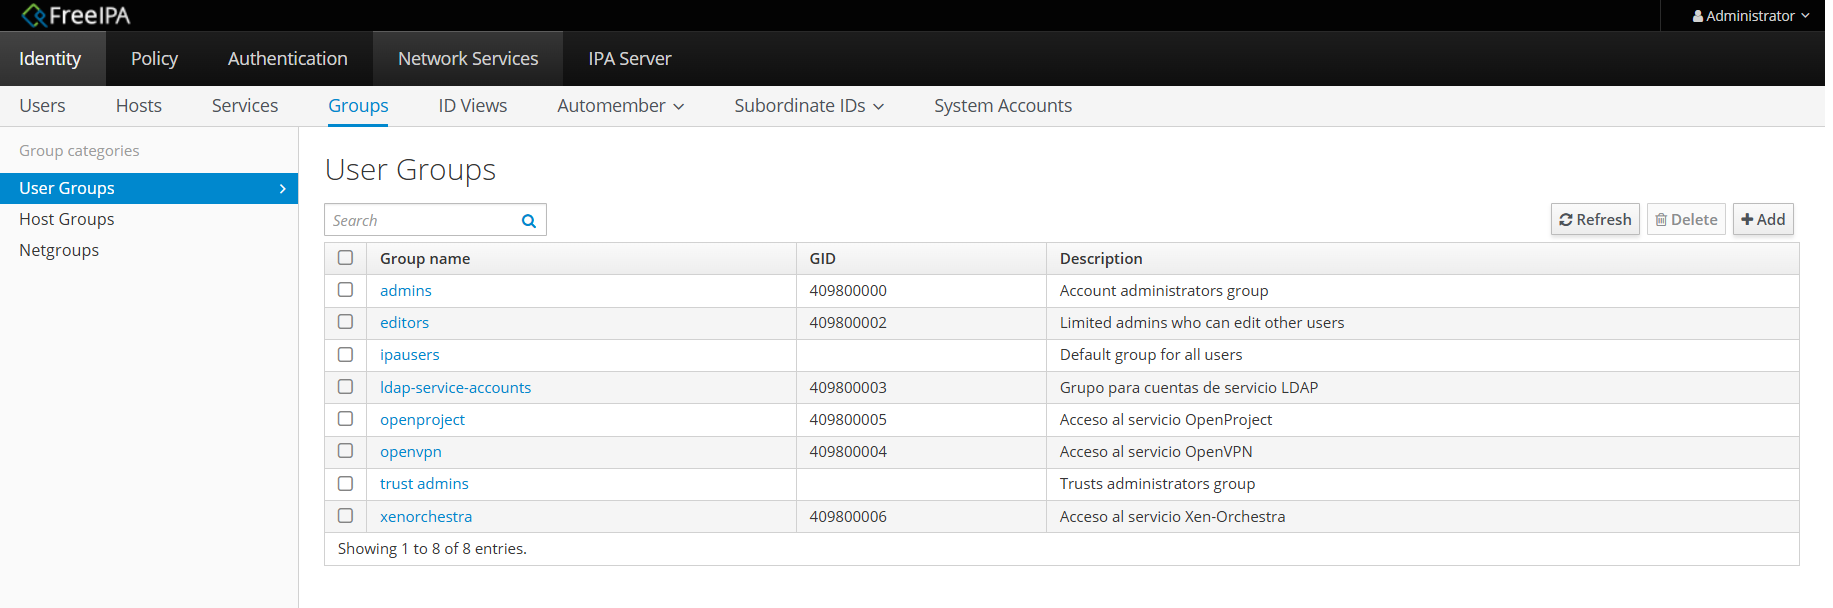
\includegraphics[width=0.85\textwidth]{imagenes/figuras/II-desarrollo-metodologico/pruebas/figura-25.png}
		      \caption{Grupos de autorización configurados en FreeIPA para los servicios integrados.}
		      \label{fig:figura-25}
	      \end{figure}

	\item \textbf{Consulta de los usuarios pertenecientes a los grupos:} Se consultó la composición de cada grupo de autorización para identificar los usuarios que se encontraban asociados a cada servicio. Esta consulta permitió establecer la relación entre las identidades gestionadas y los permisos asignados mediante los grupos. En la \autoref{fig:figura-26} se observan los usuarios del grupo openproject, en la \autoref{fig:figura-27} los del grupo openvpn, y en la \autoref{fig:figura-28} los del grupo xenorchestra.
	      \begin{figure}[H]
		      \centering
		      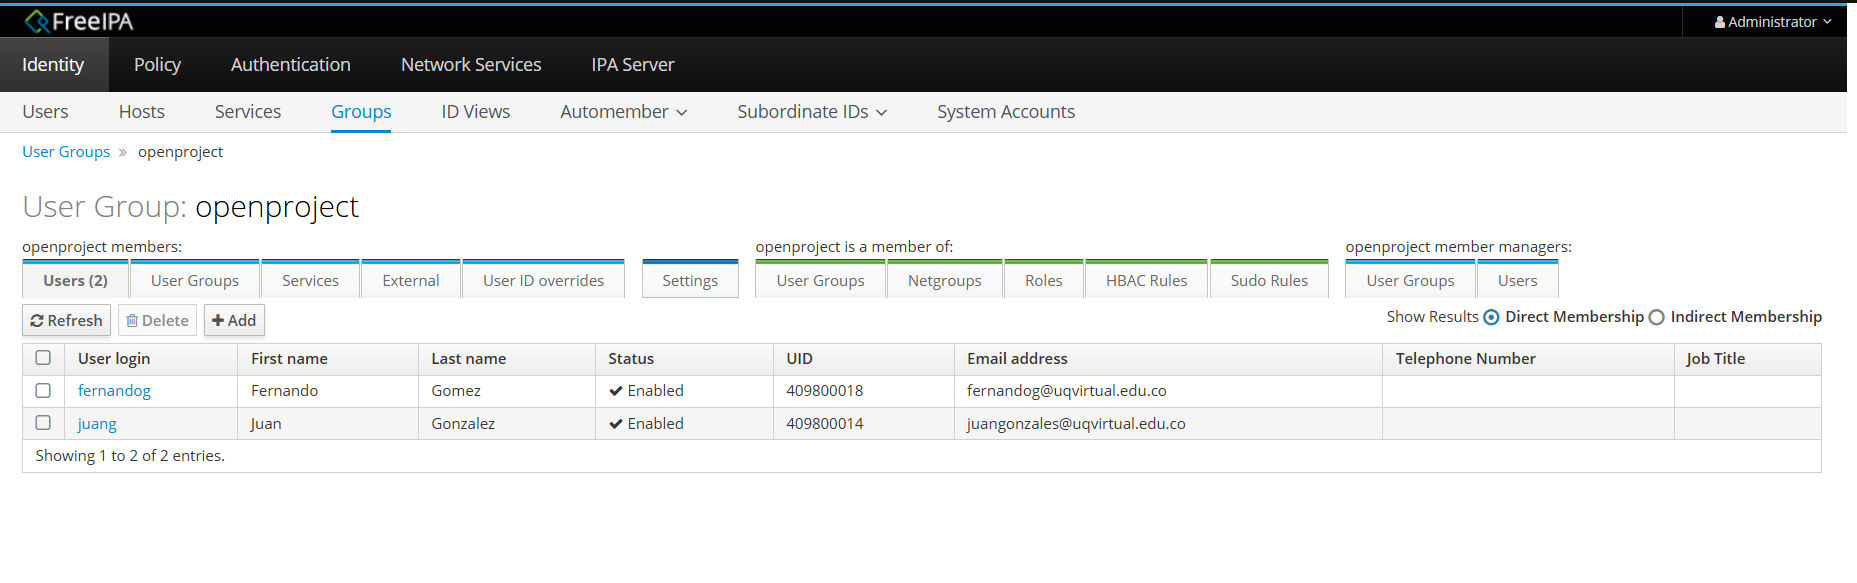
\includegraphics[width=0.85\textwidth]{imagenes/figuras/II-desarrollo-metodologico/pruebas/figura-26.png}
		      \caption{Usuarios pertenecientes al grupo de autorización openproject.}
		      \label{fig:figura-26}
	      \end{figure}

	      \begin{figure}[H]
		      \centering
		      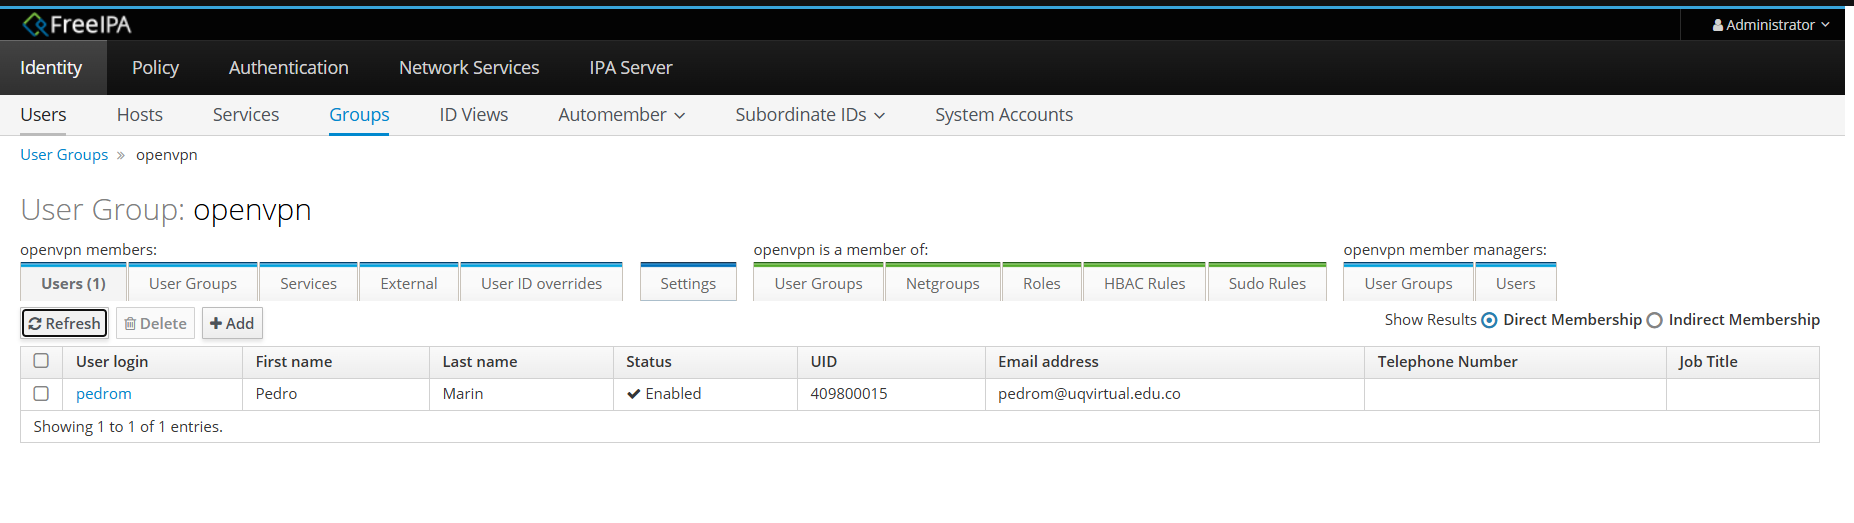
\includegraphics[width=0.85\textwidth]{imagenes/figuras/II-desarrollo-metodologico/pruebas/figura-27.png}
		      \caption{Usuarios pertenecientes al grupo de autorización openvpn.}
		      \label{fig:figura-27}
	      \end{figure}

	      \begin{figure}[H]
		      \centering
		      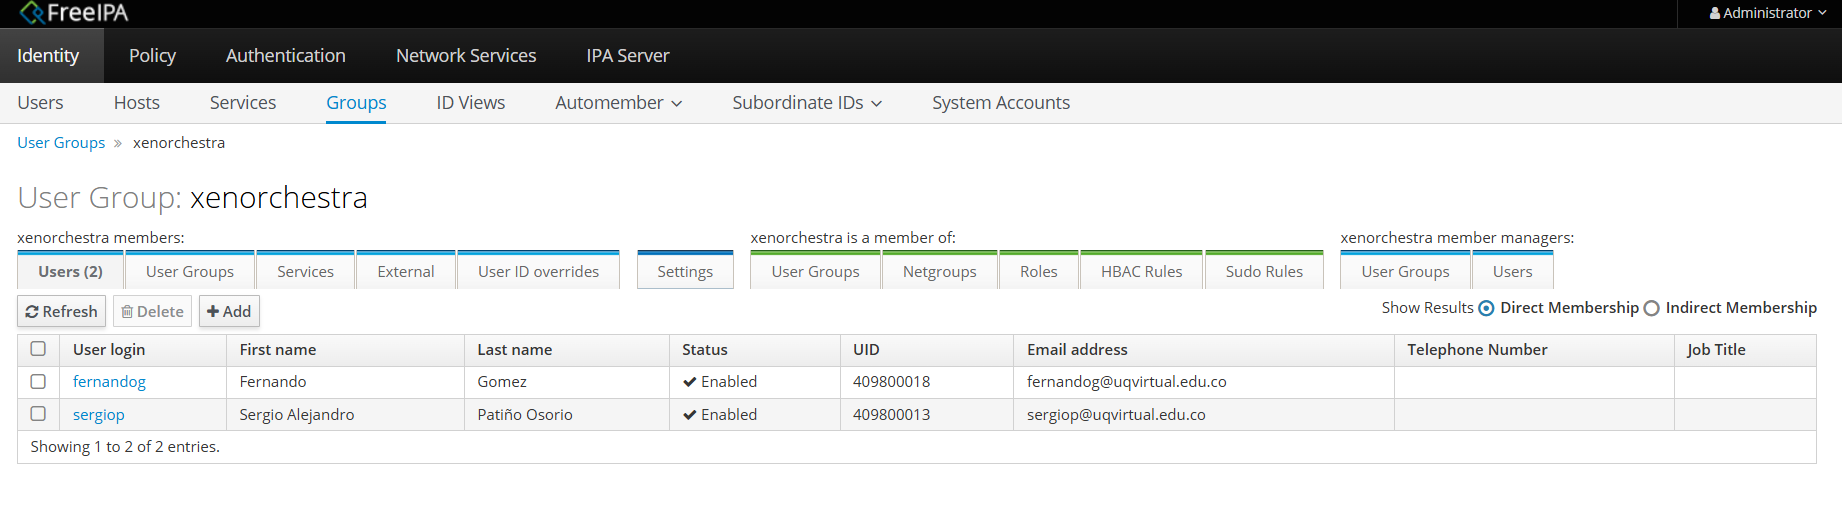
\includegraphics[width=0.85\textwidth]{imagenes/figuras/II-desarrollo-metodologico/pruebas/figura-28.png}
		      \caption{Usuarios pertenecientes al grupo de autorización xenorchestra.}
		      \label{fig:figura-28}
	      \end{figure}
\end{enumerate}
\textbf{Estado:} Cumple.\\
\textbf{Observaciones:} La prueba permitió comprobar que la configuración de grupos de FreeIPA proporciona información que puede utilizarse para revisar qué entidades tienen acceso a los servicios correspondientes a cada uno de los grupos.

\subsection{PT-07 - Replicación y sincronización del servicio de directorio}
\textbf{Requisitos asociados:}\\
\textbf{Objetivo:} Verificar que la información gestionada por el servidor principal de FreeIPA sea replicada correctamente hacia el servidor réplica y que los cambios realizados sobre las identidades se mantienen sincronizados entre ambos servidores.\\
\textbf{Resultado esperado:} Las identidades creadas o modificadas en uno de los servidores deben ser replicadas hacia el otro servidor, manteniendo consistente la información del directorio.
La creación de una cuenta en el servidor principal debe reflejarse en el servidor réplica. De igual manera, las modificaciones realizadas sobre una identidad deben propagarse entre ambos servidores de acuerdo con la configuración de replicación establecida.\\
\textbf{Precondiciones:}
\begin{itemize}
	\item El servidor principal y el servidor réplica de FreeIPA se encuentran operativos.
	\item La relación de replicación entre ambos servidores se encuentra configurada.
	\item Los servicios necesarios para la replicación se encuentran disponibles.
	\item Se dispone de una cuenta de prueba para realizar modificaciones sobre el directorio.
	\item Existe conectividad entre el servidor principal y el servidor réplica.
\end{itemize}
\textbf{Procedimiento y evidencias:}
\begin{enumerate}
	\item \textbf{Verificación de la topología de replicación:} Se consultó desde la interfaz web de administración de FreeIPA la topología configurada, con el propósito de verificar la existencia del servidor principal y del servidor réplica dentro de la infraestructura del servicio de directorio, como se presenta en la \autoref{fig:figura-29}.
	      \begin{figure}[H]
		      \centering
		      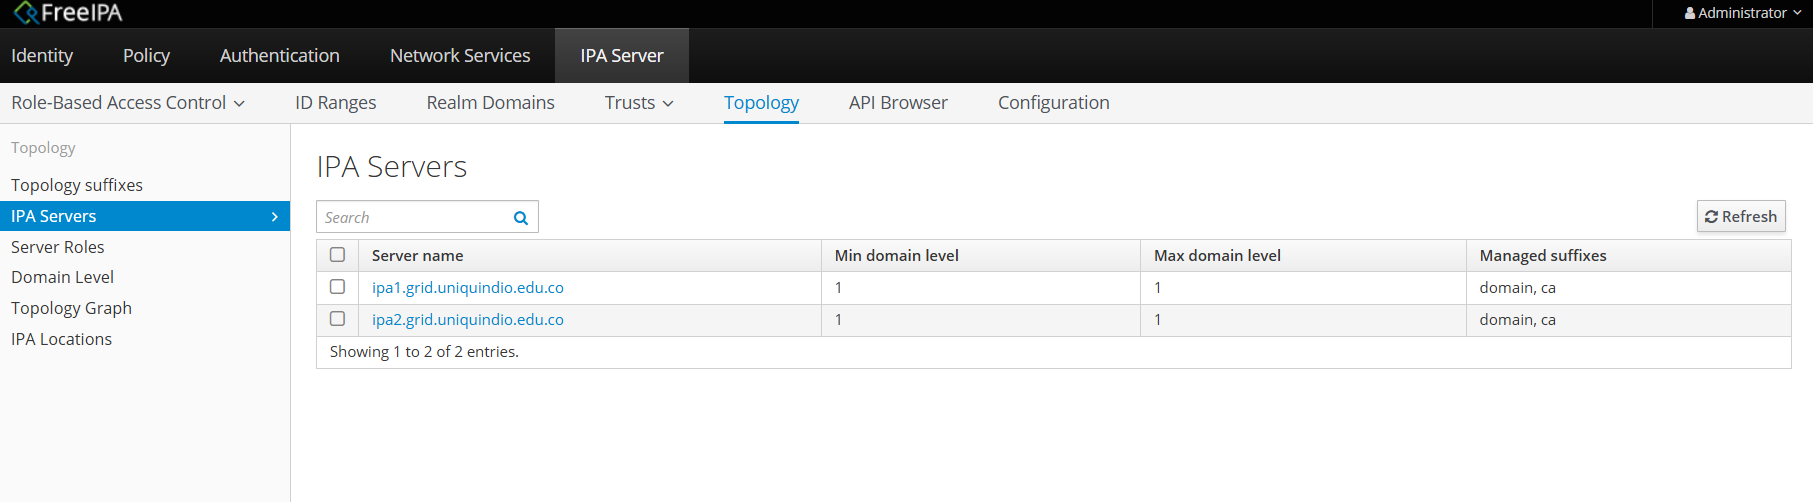
\includegraphics[width=0.85\textwidth]{imagenes/figuras/II-desarrollo-metodologico/pruebas/figura-29.png}
		      \caption{Estado de la topología de replicación de FreeIPA}
		      \label{fig:figura-29}
	      \end{figure}

	\item \textbf{Verificación inicial de la identidad:} Se seleccionó una cuenta de prueba para realizar la validación de la replicación. Desde la \ac{CLI} del servidor principal se consultó la información de la cuenta, estableciendo los atributos que posteriormente serían utilizados como referencia para comprobar su sincronización, tal como se observa en la \autoref{fig:figura-30}.
	      \begin{figure}[H]
		      \centering
		      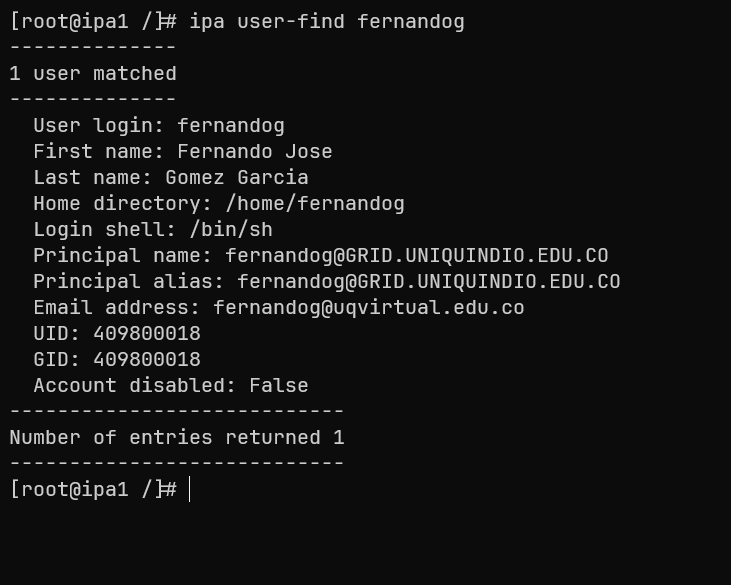
\includegraphics[width=0.85\textwidth]{imagenes/figuras/II-desarrollo-metodologico/pruebas/figura-30.png}
		      \caption{Información inicial de la cuenta de prueba consultada desde el servidor principal.}
		      \label{fig:figura-30}
	      \end{figure}

	\item \textbf{Creación o modificación de la identidad en el servidor principal:} Se realizó una operación de gestión sobre la cuenta de prueba desde el servidor principal, como se presenta en la \autoref{fig:figura-31}. Posteriormente, se consultó nuevamente la información mediante la \ac{CLI} para comprobar que el cambio hubiera sido aplicado correctamente en el servidor de origen.
	      \begin{figure}[H]
		      \centering
		      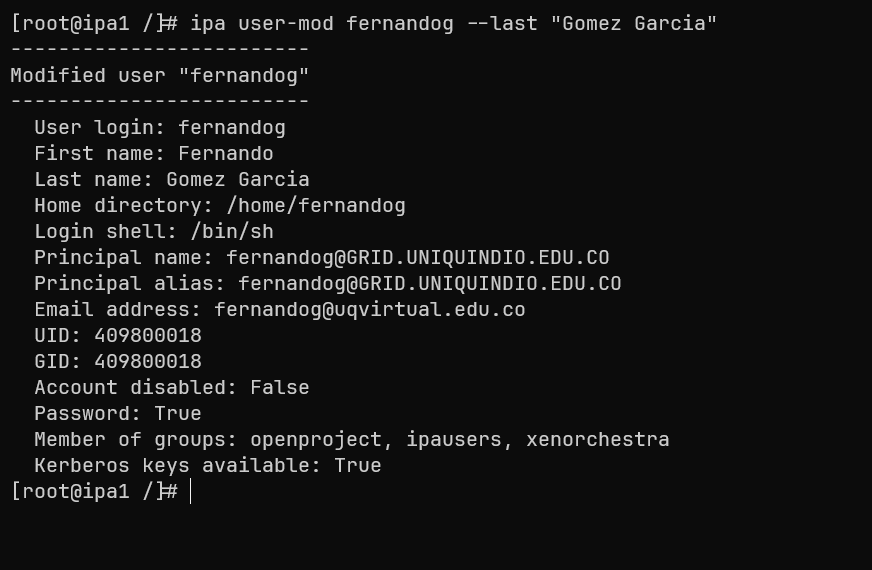
\includegraphics[width=0.85\textwidth]{imagenes/figuras/II-desarrollo-metodologico/pruebas/figura-31.png}
		      \caption{Cambio realizado sobre la cuenta de prueba desde el servidor principal.}
		      \label{fig:figura-31}
	      \end{figure}

	\item \textbf{Verificación del cambio en el servidor réplica:} Una vez realizado el cambio, se consultó desde la \ac{CLI} del servidor réplica la misma cuenta y sus atributos, con el propósito de comprobar que la información hubiera sido replicada, como se muestra en la \autoref{fig:figura-32}. La comparación de ambas consultas permitió establecer de manera directa la correspondencia entre la información existente en el servidor principal y la almacenada en el servidor réplica.
	      \begin{figure}[H]
		      \centering
		      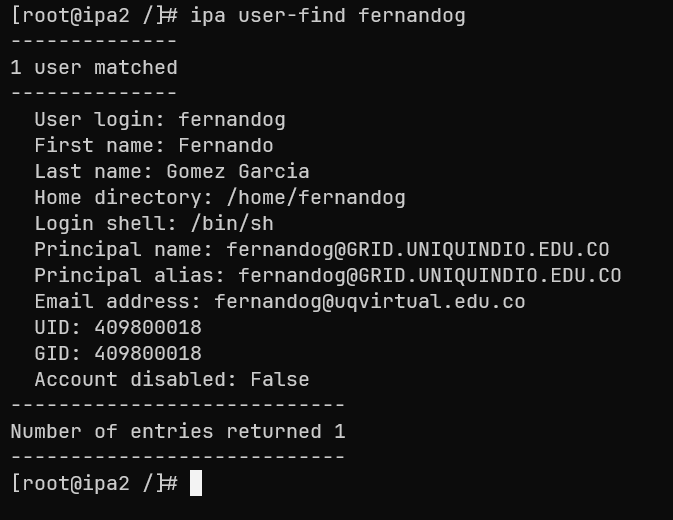
\includegraphics[width=0.85\textwidth]{imagenes/figuras/II-desarrollo-metodologico/pruebas/figura-32.png}
		      \caption{Información de la cuenta de prueba replicada en el servidor réplica.}
		      \label{fig:figura-32}
	      \end{figure}

	\item \textbf{Validación de la replicación en sentido inverso:} Se realizó una modificación sobre una identidad desde el servidor réplica y posteriormente se consultó la misma información desde el servidor principal, tal como se presenta en la \autoref{fig:figura-33}. Esto permitió comprobar el comportamiento de la replicación en ambos sentidos.
	      \begin{figure}[H]
		      \centering
		      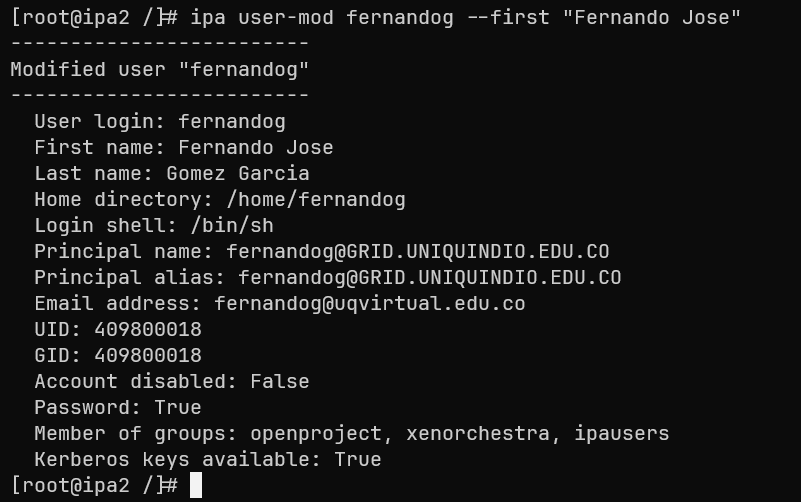
\includegraphics[width=0.85\textwidth]{imagenes/figuras/II-desarrollo-metodologico/pruebas/figura-33.png}
		      \caption{Cambio realizado desde el servidor réplica y reflejado en el servidor principal.}
		      \label{fig:figura-33}
	      \end{figure}
\end{enumerate}
\textbf{Estado:} Cumple.\\
\textbf{Observaciones:} La prueba permitió comprobar el funcionamiento de la replicación entre el servidor principal y el servidor réplica de FreeIPA, verificando que los cambios realizados sobre las identidades fueran propagados entre ambos servidores. Esta prueba constituye además la base para las pruebas posteriores relacionadas con la continuidad y recuperación del servicio de directorio.

\subsection{PT-08 - Continuidad ante falla del servidor principal}
\textbf{Requisitos asociados:}\\
\textbf{Objetivo:} Verificar la continuidad del servicio de directorio ante la indisponibilidad del servidor principal de FreeIPA, comprobando que el servidor réplica pueda mantener la disponibilidad de las identidades y atender las operaciones de autenticación de los servicios integrados.\\
\textbf{Resultado esperado:} Ante la indisponibilidad del servidor principal, el servidor réplica debe permanecer operativo y conservar la información de las identidades previamente sincronizadas.
La condición de falla no debe impedir la autenticación ni el acceso a los servicios integrados cuando estos pueden continuar utilizando el servidor réplica disponible.
Una vez restablecido el servidor principal, ambos servidores deben recuperar su funcionamiento normal y mantener la configuración de replicación establecida.\\
\textbf{Precondiciones:}
\begin{itemize}
	\item El servidor principal y el servidor réplica de FreeIPA se encuentran operativos.
	\item La replicación entre ambos servidores se encuentra funcionando correctamente.
	\item Las identidades utilizadas para la prueba se encuentran sincronizadas en ambos servidores.
	\item Los servicios integrados se encuentran configurados para utilizar el servicio de directorio.
	\item Se dispone de una cuenta de prueba con autorización para acceder al servicio utilizado durante la validación.
	\item Se ha comprobado previamente el funcionamiento normal del acceso antes de provocar la falla.
\end{itemize}
\textbf{Procedimiento y evidencias:}
\begin{enumerate}
	\item \textbf{Verificación del funcionamiento normal:} Se verificó inicialmente el estado operativo de los servidores principal y réplica y se realizó una autenticación con la cuenta de prueba para establecer el funcionamiento normal del servicio antes de generar la condición de falla, como se observa en la \autoref{fig:figura-34}.
	      \begin{figure}[H]
		      \centering
		      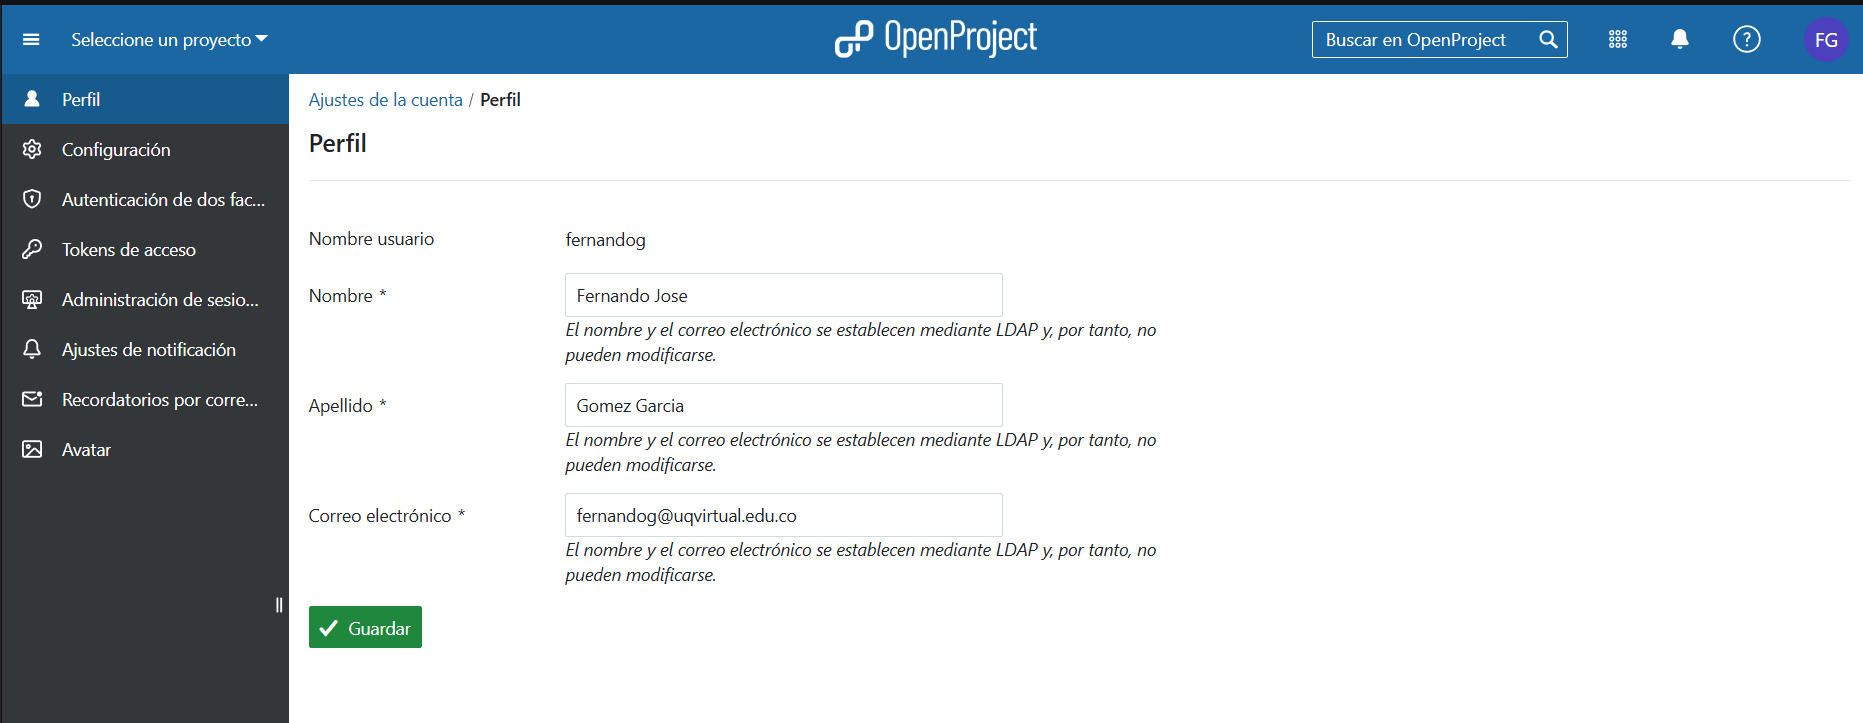
\includegraphics[width=0.85\textwidth]{imagenes/figuras/II-desarrollo-metodologico/pruebas/figura-34.png}
		      \caption{Estado operativo de los servidores y autenticación previa a la falla.}
		      \label{fig:figura-34}
	      \end{figure}

	\item \textbf{Indisponibilidad del servidor principal:} Se interrumpió de manera controlada la disponibilidad del servidor principal de FreeIPA, simulando una condición de falla del servidor, como se presenta en la \autoref{fig:figura-35}. Una vez aplicada la condición, se verificó que el servidor principal deja de estar disponible para las operaciones del servicio de directorio.
	      \begin{figure}[H]
		      \centering
		      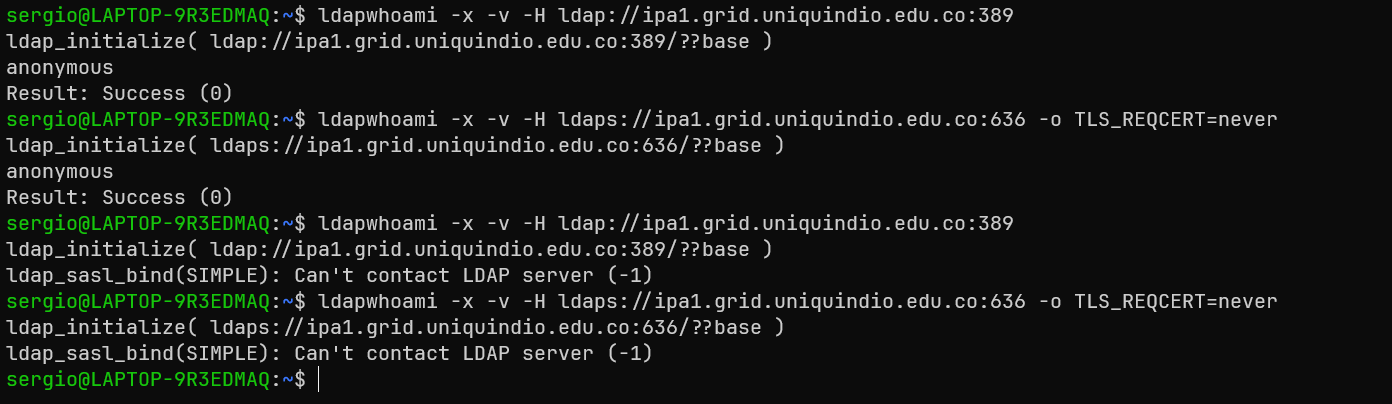
\includegraphics[width=0.85\textwidth]{imagenes/figuras/II-desarrollo-metodologico/pruebas/figura-35.png}
		      \caption{Indisponibilidad controlada del servidor principal de FreeIPA.}
		      \label{fig:figura-35}
	      \end{figure}

	\item \textbf{Verificación de la disponibilidad del servidor réplica:} Con el servidor principal fuera de servicio, se verificó el estado del servidor réplica para comprobar que permaneciera operativo y que contiene la información de las identidades previamente replicadas, tal como se observa en la \autoref{fig:figura-36}.
	      \begin{figure}[H]
		      \centering
		      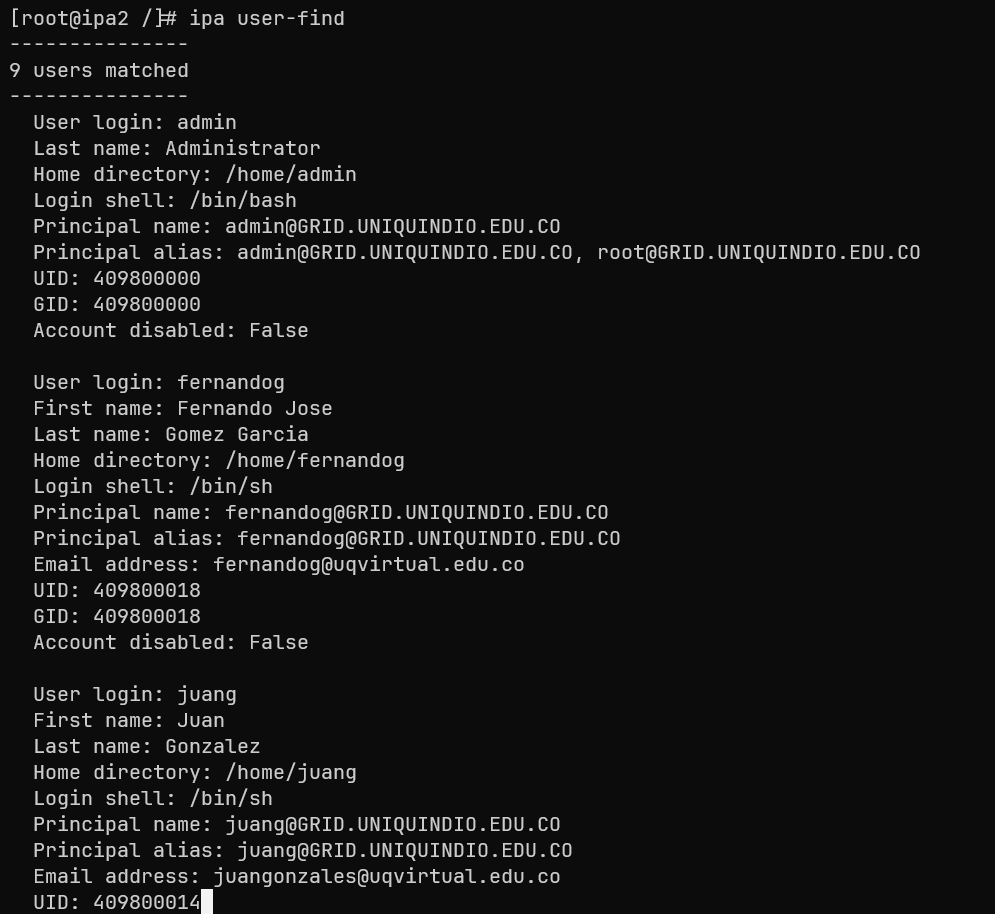
\includegraphics[width=0.85\textwidth]{imagenes/figuras/II-desarrollo-metodologico/pruebas/figura-36.png}
		      \caption{Estado operativo del servidor réplica durante la indisponibilidad del servidor principal.}
		      \label{fig:figura-36}
	      \end{figure}

	\item \textbf{Validación de la autenticación durante la falla:} Mientras el servidor principal permaneció indisponible, se realizó un nuevo intento de autenticación utilizando la cuenta de prueba en el servicio integrado. Se verificó si el servicio podía continuar utilizando la información disponible en el servidor réplica, como se presenta en la \autoref{fig:figura-37}.
	      \begin{figure}[H]
		      \centering
		      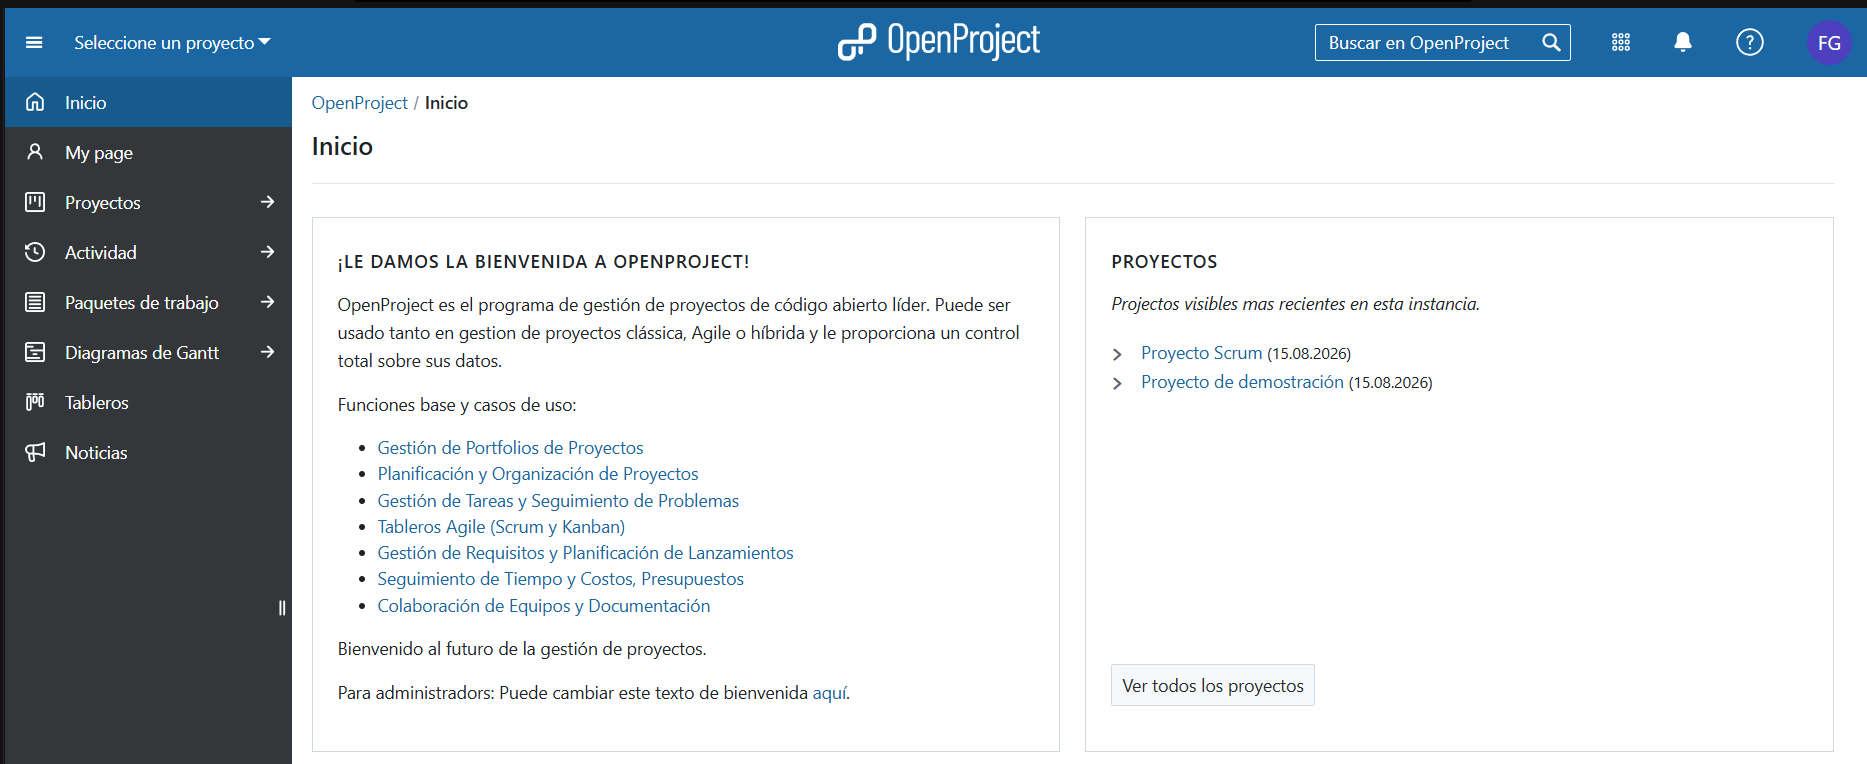
\includegraphics[width=0.85\textwidth]{imagenes/figuras/II-desarrollo-metodologico/pruebas/figura-37.png}
		      \caption{Autenticación realizada durante la indisponibilidad del servidor principal.}
		      \label{fig:figura-37}
	      \end{figure}

	\item \textbf{Restablecimiento del servidor principal:} Una vez finalizada la validación, se restableció la disponibilidad del servidor principal y se verificó nuevamente el estado de la infraestructura de FreeIPA, tal como se muestra en la \autoref{fig:figura-38}.
	      \begin{figure}[H]
		      \centering
		      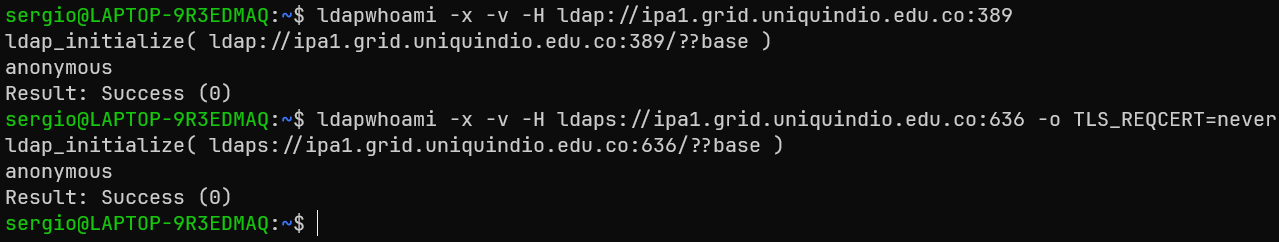
\includegraphics[width=0.85\textwidth]{imagenes/figuras/II-desarrollo-metodologico/pruebas/figura-38.png}
		      \caption{Recuperación del servidor principal y estado de la infraestructura después de la prueba.}
		      \label{fig:figura-38}
	      \end{figure}
\end{enumerate}
\textbf{Estado:} Cumple.\\
\textbf{Observaciones:} La prueba permite comprobar el comportamiento de la infraestructura ante la indisponibilidad del servidor principal, utilizando el servidor réplica como componente disponible del servicio de directorio. Los resultados obtenidos complementan la prueba PT-07, ya que mientras esta verificó la sincronización de la información entre los servidores, PT-08 evaluó la continuidad del servicio ante la falla de uno de ellos.

\subsection{PT-09 - Recuperación y resincronización del servicio de directorio}
\textbf{Requisitos asociados:}\\
\textbf{Objetivo:} Verificar la recuperación del servidor principal después de una condición de falla y comprobar que, una vez restablecida la comunicación entre los servidores de FreeIPA, la información del directorio se encuentre nuevamente sincronizada.\\
\textbf{Resultado esperado:} Después de restablecer el servidor principal, este debe reincorporarse correctamente a la topología de FreeIPA y recuperar la comunicación con el servidor réplica.
Los cambios realizados sobre las identidades durante la indisponibilidad del servidor principal deben ser sincronizados una vez restablecida la comunicación entre ambos servidores. Al finalizar la prueba, la información correspondiente a las identidades utilizadas debe encontrarse consistente en ambos servidores y la replicación debe permanecer operativa.\\
\textbf{Precondiciones:}
\begin{itemize}
	\item El servidor principal y el servidor réplica de FreeIPA se encuentran configurados como réplicas.
	\item La replicación se encuentra operativa antes de iniciar la prueba.
	\item El servidor principal ha sido previamente sometido a una condición de indisponibilidad controlada.
	\item El servidor réplica permanece operativo durante la prueba.
	\item Se dispone de una cuenta de prueba para generar cambios durante la indisponibilidad del servidor principal.
	\item Se dispone de acceso administrativo para consultar el estado de la replicación.
\end{itemize}
\textbf{Procedimiento y evidencias:}
\begin{enumerate}
	\item \textbf{Verificación del estado previo a la recuperación:} Se verificó que el servidor réplica permaneciera operativo y que el servidor principal se encuentre indisponible, como se presenta en la \autoref{fig:figura-39}.
	      \begin{figure}[H]
		      \centering
		      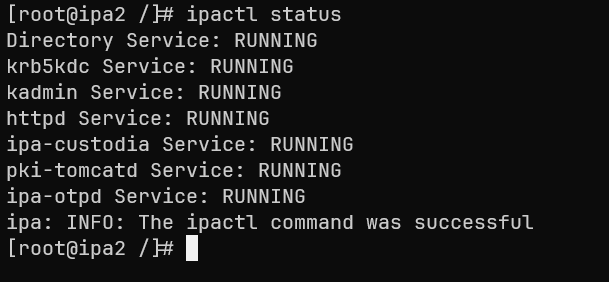
\includegraphics[width=0.85\textwidth]{imagenes/figuras/II-desarrollo-metodologico/pruebas/figura-39.png}
		      \caption{Estado de los servidores antes de iniciar la recuperación del servidor principal.}
		      \label{fig:figura-39}
	      \end{figure}

	\item \textbf{Generación de un cambio durante la indisponibilidad:} Mientras el servidor principal permaneció fuera de servicio, se realizó una modificación sobre una identidad desde el servidor réplica, tal como se observa en la \autoref{fig:figura-40}. El cambio se utilizó como referencia para comprobar posteriormente la sincronización de la información una vez restablecido el servidor principal.
	      \begin{figure}[H]
		      \centering
		      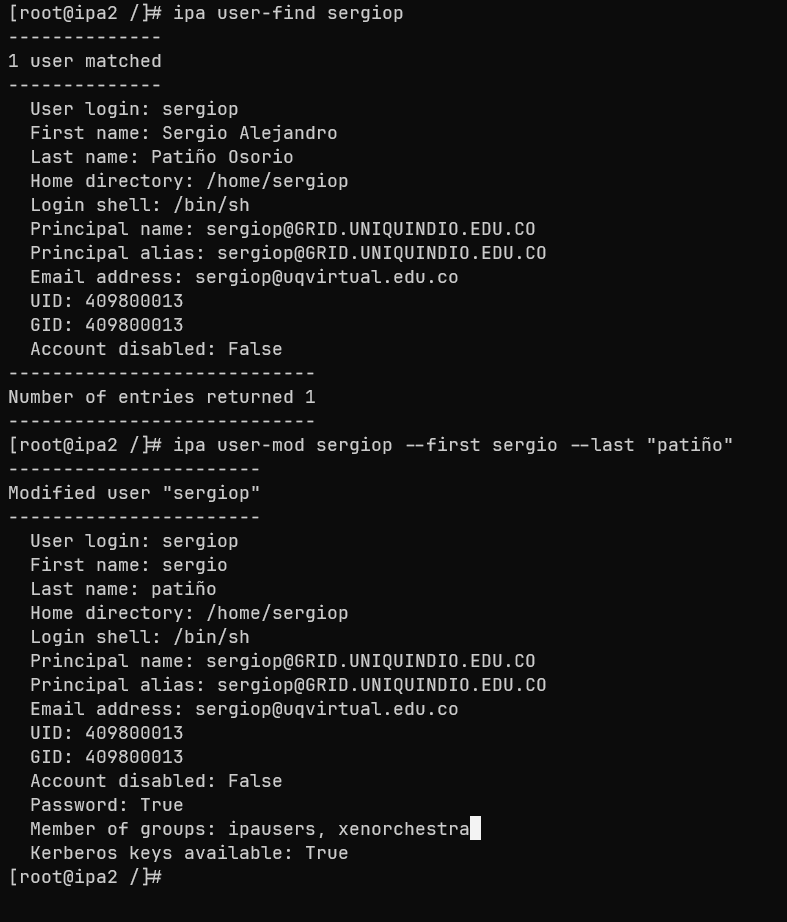
\includegraphics[width=0.85\textwidth]{imagenes/figuras/II-desarrollo-metodologico/pruebas/figura-40.png}
		      \caption{Modificación realizada sobre la identidad desde el servidor réplica durante la indisponibilidad del servidor principal.}
		      \label{fig:figura-40}
	      \end{figure}

	\item \textbf{Restablecimiento del servidor principal:} Se restableció la disponibilidad del servidor principal y se verificó que los servicios necesarios para la operación de FreeIPA se encontrarán nuevamente activos, como se presenta en la \autoref{fig:figura-41}.
	      \begin{figure}[H]
		      \centering
		      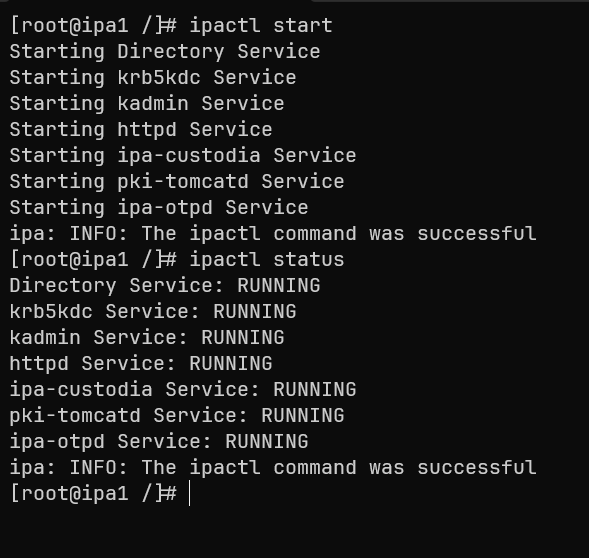
\includegraphics[width=0.85\textwidth]{imagenes/figuras/II-desarrollo-metodologico/pruebas/figura-41.png}
		      \caption{Restablecimiento del servidor principal de FreeIPA.}
		      \label{fig:figura-41}
	      \end{figure}

	\item \textbf{Verificación de la información modificada:} Se consultó desde el servidor principal la identidad que había sido modificada durante su indisponibilidad. Se verificó que el cambio realizado desde el servidor réplica se encontrase reflejado en el servidor principal, tal como se muestra en la \autoref{fig:figura-42}.
	      \begin{figure}[H]
		      \centering
		      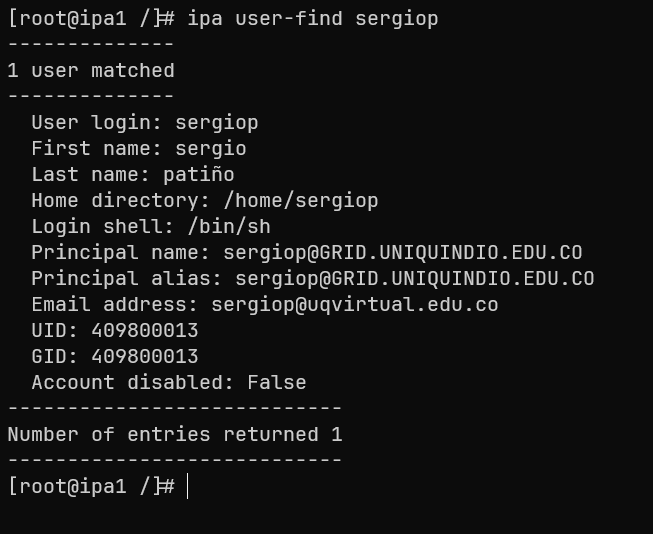
\includegraphics[width=0.85\textwidth]{imagenes/figuras/II-desarrollo-metodologico/pruebas/figura-42.png}
		      \caption{Cambio realizado durante la falla y posteriormente sincronizado en el servidor principal.}
		      \label{fig:figura-42}
	      \end{figure}

	\item \textbf{Validación de la sincronización posterior:} Finalmente, se verificó que ambos servidores conservaran la misma información de la identidad utilizada durante la prueba y que la replicación continuaba operativa después de la recuperación del servidor principal, como se presenta en la \autoref{fig:figura-43}.
	      \begin{figure}[H]
		      \centering
		      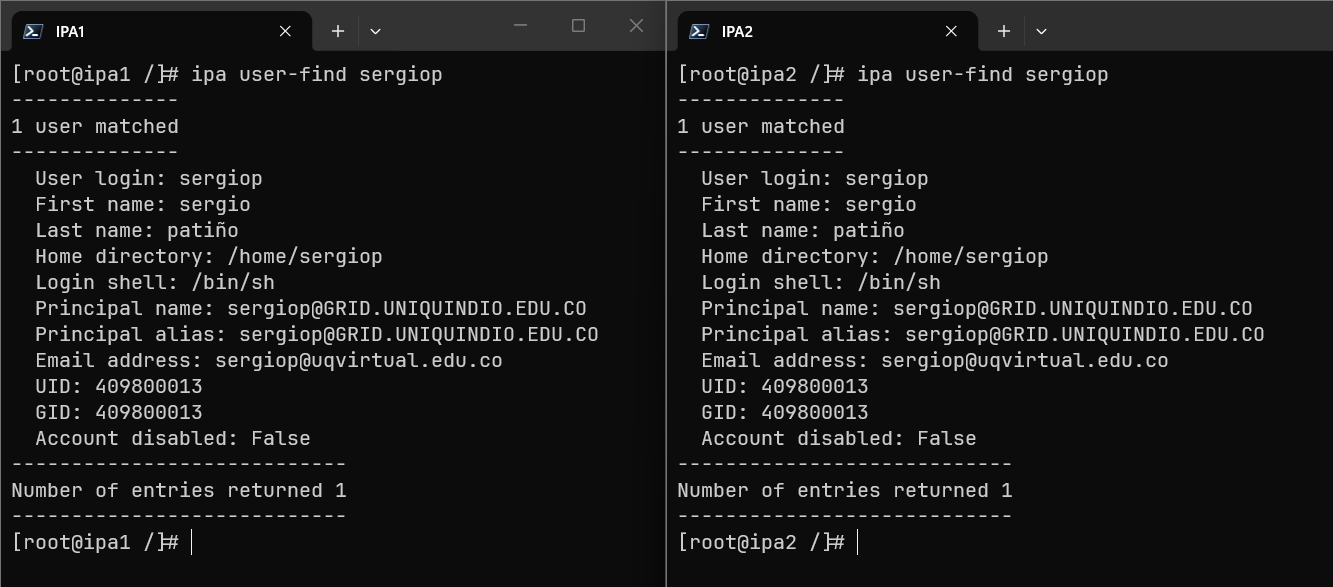
\includegraphics[width=0.85\textwidth]{imagenes/figuras/II-desarrollo-metodologico/pruebas/figura-43.png}
		      \caption{Información sincronizada entre el servidor principal y el servidor réplica después de la recuperación.}
		      \label{fig:figura-43}
	      \end{figure}
\end{enumerate}
\textbf{Estado:} Cumple.\\
\textbf{Observaciones:} La prueba permitió verificar el comportamiento del servicio de directorio después de la recuperación del servidor principal. A diferencia de PT-08, que evaluó la continuidad del servicio durante la indisponibilidad, esta prueba se centró en la recuperación de la infraestructura y la re-sincronización de la información después de restablecer el servidor.
En conjunto, PT-07, PT-08 y PT-09 permitieron evaluar la replicación, la continuidad ante una falla y la recuperación posterior del servicio de directorio sin repetir el mismo escenario de validación.

\section{Evaluación del cumplimiento de requisitos}
Una vez finalizada la ejecución de los casos de prueba, se realizó la evaluación del cumplimiento de los requisitos establecidos para la solución. Para ello, se contrastaron los resultados obtenidos y las evidencias recopiladas durante las pruebas con las condiciones definidas para cada requisito.

El resultado de esta evaluación se clasificó en tres categorías: cumple, cuando las funcionalidades requeridas fueron implementadas y verificadas mediante las pruebas; cumplimiento parcial, cuando se implementó una parte del requisito, pero alguna de sus características no pudo ser incorporada dentro de la arquitectura establecida; y no cumple, cuando la funcionalidad requerida no fue implementada en la solución. Los resultados consolidados se presentan en la \autoref{tab:evaluacion-requisitos}.

\begingroup
\fontsize{8.5pt}{9.5pt}\selectfont
\renewcommand{\arraystretch}{1.3}
\setlength{\tabcolsep}{4pt}

\begin{longtable}{|
	>{\raggedright\arraybackslash}p{1.2cm}|
	>{\raggedright\arraybackslash}p{4.0cm}|
	>{\raggedright\arraybackslash}p{2.3cm}|
	>{\raggedright\arraybackslash}p{2.0cm}|
	>{\raggedright\arraybackslash}p{4.0cm}|}

	\caption{Evaluación del cumplimiento de requisitos}
	\label{tab:evaluacion-requisitos}
	\\
	\hline
	\rowcolor[gray]{0.85}
	\textbf{ID}                &
	\textbf{Requisito}         &
	\textbf{Pruebas asociadas} &
	\textbf{Resultado}         &
	\textbf{Observaciones}
	\\
	\hline
	\endfirsthead

	\caption{Evaluación del cumplimiento de requisitos (continuación)}
	\\
	\hline
	\rowcolor[gray]{0.85}
	\textbf{ID}                &
	\textbf{Requisito}         &
	\textbf{Pruebas asociadas} &
	\textbf{Resultado}         &
	\textbf{Observaciones}
	\\
	\hline
	\endhead

	R-01                       & Gestionar centralizadamente las identidades y mantener autorización diferenciada por sistema.                                          & PT-01, PT-02                  & Cumple               & Se verificó la autenticación centralizada y la aplicación de autorización diferenciada mediante grupos.                                                                         \\ \hline
	R-02                       & Gestionar el ciclo de vida de las cuentas, incluyendo creación, actualización, habilitación, deshabilitación, revocación y expiración. & PT-03                         & Cumple               & Se verificaron las operaciones de gestión del ciclo de vida contempladas en la implementación.                                                                                  \\ \hline
	R-03                       & Definir y aplicar políticas de seguridad para usuarios y credenciales.                                                                 & PT-04                         & Cumple               & Se verificó la aplicación de las políticas de credenciales configuradas.                                                                                                        \\ \hline
	R-04                       & Controlar y monitorear los accesos y facilitar la revisión de permisos.                                                                & PT-02, PT-06                  & Cumple               & Se verificó el control de acceso mediante grupos y la revisión de los permisos asociados.                                                                                       \\ \hline
	R-05                       & Registrar actividades relevantes de gestión de identidades y accesos para fines de auditoría.                                          & PT-05                         & Cumple               & Se verificó que una operación de gestión de identidad generara un registro que permite identificar la actividad realizada.                                                      \\ \hline
	R-06                       & Fortalecer la autenticación mediante políticas de credenciales y mecanismos adicionales de autenticación.                              & PT-04                         & Cumplimiento parcial & Se implementaron políticas de credenciales, pero la integración de \acs{MFA} con los servicios mediante \acs{LDAP} no fue posible dentro de la arquitectura implementada.       \\ \hline
	R-07                       & Proporcionar mecanismos seguros de recuperación o restablecimiento de credenciales.                                                    &                               & No cumple            & FreeIPA no proporciona un mecanismo nativo de recuperación de contraseña mediante autoservicio. La incorporación de alternativas externas quedó fuera del alcance del proyecto. \\ \hline
	R-08                       & Permitir la evolución y ampliación del servicio ante la incorporación de nuevos sistemas o activos.                                    & PT-01, pruebas de integración & Cumple               & La integración de los tres servicios mediante el directorio centralizado evidencia la capacidad de incorporar sistemas al servicio de directorio.                               \\ \hline
\end{longtable}
\endgroup
\normalsize

\subsection{Consideraciones y limitaciones}
Durante la ejecución de las pruebas se tuvieron en cuenta las condiciones del entorno de implementación y el alcance establecido para la solución. Estas consideraciones permitieron delimitar los resultados obtenidos y establecer las condiciones bajo las cuales se evaluó el cumplimiento de los requisitos.

Las pruebas se realizaron sobre el entorno compuesto por el servidor principal, el servidor réplica de FreeIPA y el balanceador HAProxy, junto con los servicios integrados OpenVPN, OpenProject y Xen Orchestra.

Para la ejecución de las pruebas se utilizaron tanto la interfaz web de administración de FreeIPA como la interfaz de línea de comandos. La interfaz web se empleó principalmente para evidenciar elementos cuya representación gráfica facilita su interpretación, como la topología de replicación. Por su parte, la \ac{CLI} se utilizó para las operaciones y consultas que requerían contrastar directamente la información entre el servidor principal y el servidor réplica, especialmente en las pruebas de replicación, continuidad y recuperación.

Las evidencias se integraron directamente con el procedimiento de cada caso de prueba. De esta manera, cada evidencia se relaciona con la actividad que permitió obtenerla, facilitando la trazabilidad entre las acciones ejecutadas y los resultados observados. Asimismo, cuando una actividad ya había sido validada en una prueba anterior, sus resultados se utilizaron como antecedente en pruebas posteriores para evitar la repetición innecesaria de procedimientos y evidencias.

\subsubsection{Limitaciones}
Una de las limitaciones identificadas corresponde al requisito R-06, relacionado con el fortalecimiento de la autenticación mediante políticas de credenciales y mecanismos adicionales de autenticación. La autenticación multifactor se contempló dentro del alcance del proyecto; sin embargo, la integración de OpenVPN, OpenProject y Xen Orchestra se realizó mediante \ac{LDAP}, y las implementaciones \ac{LDAP} utilizadas por estos servicios no contemplan, dentro de este mecanismo de integración, el uso de la autenticación multifactor proporcionada por FreeIPA. Por tanto, aunque FreeIPA dispone de capacidades relacionadas con mecanismos adicionales de autenticación, estas no pudieron incorporarse a los tres servicios mediante la arquitectura implementada.

La incorporación de autenticación multifactor directamente en los servicios podría requerir mecanismos de integración adicionales o componentes específicos de cada plataforma, lo que implicaría ampliar la arquitectura planteada y utilizar servicios adicionales. Por este motivo, dicha alternativa se mantiene fuera del alcance de la implementación realizada. En consecuencia, la evaluación de R-06 debe distinguir entre las políticas de credenciales implementadas y el mecanismo adicional de autenticación que no pudo integrarse mediante \ac{LDAP}.

Otra limitación corresponde al requisito R-07, relacionado con la recuperación o restablecimiento de credenciales. La implementación permite al usuario modificar su contraseña cuando dispone de la credencial vigente; sin embargo, no proporciona un mecanismo de recuperación de contraseña cuando esta ha sido olvidada. Esta limitación corresponde a una decisión del propio proyecto FreeIPA: su documentación señala que el restablecimiento de contraseña mediante autoservicio no forma parte de las funcionalidades principales de gestión de usuarios y que los usuarios que olvidan sus credenciales deben recurrir al administrador o a la mesa de ayuda, previa verificación de su identidad \citep{FreeIPAReset2026}.

La documentación de FreeIPA también señala que determinados mecanismos habituales de recuperación, como las preguntas de seguridad o el restablecimiento mediante correo electrónico, pueden introducir vulnerabilidades asociadas, por ejemplo, a ingeniería social o a la transmisión insegura de información. Debido a estas consideraciones, el equipo de FreeIPA no contempla incorporar este tipo de mecanismos dentro de las funcionalidades principales de la plataforma \citep{FreeIPAReset2026}; en su lugar, plantea que los administradores que requieran esta capacidad desarrollen e integren soluciones propias de restablecimiento mediante la \ac{API} interna o la interfaz \ac{LDAP} del sistema, adaptadas a los requerimientos de seguridad de cada infraestructura.
